%% ============================================================
%%  Battery Storage and Electricity Price Convergence:
%%  A Threshold Vector Error-Correction Analysis
%%  of the South Australian–Victorian Market
%% ============================================================
\documentclass[12pt,a4paper]{article}

%% --- Packages ---
\usepackage[british]{babel}
\usepackage{csquotes}
\usepackage[
  style=authoryear,
  backend=biber,
  giveninits=true,
  terseinits=true,
  uniquename=init,
  uniquelist=false,
  maxcitenames=2,
  maxbibnames=99,
  dashed=false,
  natbib=true,
  urldate=long,
  useprefix=true
]{biblatex}
\addbibresource{references.bib}

%% --- Strict Harvard (Cite Them Right) formatting overrides ---
% Year in parentheses with no trailing period
\renewcommand*{\nameyeardelim}{\addspace}
% Remove "In:" prefix before journal/book title
\renewbibmacro{in:}{}
% Article / chapter titles in single quotes, sentence case
\DeclareFieldFormat[article,inbook,incollection,inproceedings,thesis,unpublished,misc,online,report]{title}{\mkbibquote{#1\isdot}}
\DeclareFieldFormat{citetitle}{\mkbibquote{#1\isdot}}
% Book / journal titles in italics
\DeclareFieldFormat[book,manual,periodical,report,thesis]{title}{\mkbibemph{#1}}
% Volume in bold, issue in parentheses: 38(3)
\DeclareFieldFormat[article,periodical]{volume}{\textbf{#1}}
\DeclareFieldFormat[article,periodical]{number}{(#1)}
\renewbibmacro*{volume+number+eid}{%
  \printfield{volume}%
  \setunit*{\addnbspace}%
  \printfield{number}%
  \setunit{\addcomma\space}%
  \printfield{eid}}
% Pages with pp. prefix
\DeclareFieldFormat{pages}{pp.~#1}
% Single quote style
\DeclareQuoteAlias{british}{english}

\usepackage[margin=2.5cm]{geometry}
\usepackage{setspace}
\usepackage{amsmath,amssymb}
\usepackage{booktabs}
\usepackage{siunitx}
\usepackage[font=small,labelfont=bf]{caption}
\usepackage{threeparttable}
\usepackage{array}
\usepackage{graphicx}
\graphicspath{{../results/}}
\usepackage{rotating}
\usepackage{hyperref}
\usepackage{microtype}
\usepackage{lmodern}
\usepackage{pdflscape}

\hypersetup{
  colorlinks=true,
  linkcolor=black,
  citecolor=black,
  urlcolor=black
}

\onehalfspacing

%% --- Convenience commands ---
\newcommand{\ect}{\mathit{ECT}}
\newcommand{\dsa}{\Delta p^{\mathrm{SA}}}
\newcommand{\dvic}{\Delta p^{\mathrm{VIC}}}
\newcolumntype{R}[1]{>{\raggedleft\arraybackslash}p{#1}}
\newcolumntype{L}[1]{>{\raggedright\arraybackslash}p{#1}}
\newcolumntype{C}[1]{>{\centering\arraybackslash}p{#1}}

%% ============================================================
\begin{document}

\begin{titlepage}
  \centering
  \vspace*{3.0cm}
  {\LARGE\bfseries Battery Storage and Electricity Price Convergence\par}
  \vspace{0.6cm}
  {\Large\bfseries A Threshold Vector Error-Correction Analysis\par}
  {\Large\bfseries of the South Australian--Victorian Market\par}
  \vspace{2.5cm}
  {\large Tim Louis Wilken\par}
  \vspace{0.4cm}
  {\large 2026\par}
  \vfill
\end{titlepage}

\clearpage
\begin{center}
  \begin{abstract}
    \noindent
    This paper investigates whether battery energy storage systems (BESS)
    causally dampen wholesale electricity price spikes in South Australia (SA),
    exploiting the rapid 4.7-fold expansion in installed capacity
    (271--1{,}282~MWh) over 2023--2025.  A rigorous pre-estimation diagnostic
    sequence establishes the stochastic foundation for the core model: KPSS
    tests are preferred over ADF and Phillips--Perron for assessing level
    stationarity: the literature cautions that price spikes (additive outliers)
    bias ADF-type inference towards rejection of the unit root null, while KPSS
    reverses the null hypothesis to provide a more reliable guide.  KPSS
    rejects level stationarity for both price series; Johansen cointegration
    identifies a single long-run relationship
    ($\ect_t = p_t^{SA} - 1.2103\,p_t^{VIC}$); and the Hansen--Seo two-threshold
    bootstrap selects a three-regime TVECM ($\hat{\gamma}_{L} = -\$45.80$,
    $\hat{\gamma}_{U} = +\$20.02$/MWh, $p = 0.030$) over simpler alternatives.
    SA prices correct toward equilibrium exclusively in the spike regime
    (half-life 0.8~hours).  A triple identification strategy (contemporaneous
    OLS, predetermined regressors, and two-stage least squares with a
    capacity-normalised state-of-charge instrument validated by a novel
    commissioning-event instrument, $Z^{newcap}$, Sargan $p = 0.174$) shows
    that the OLS battery-discharge coefficient in the spike regime
    ($+1.20^{***}$) reverses sign under predetermined regressors ($-0.19$,
    $n.s.$), the preferred estimator for this regime given that the Wu-Hausman
    test does not reject exogeneity ($p = 0.731$).  The statistically
    insignificant point estimate is consistent with a small or zero marginal
    causal effect, though the wide confidence interval
    (approximately $[-0.53,\;+0.15]$) precludes a precise conclusion; the
    economic interpretation rests on converging evidence from the
    capacity-interaction model and rolling-threshold analysis rather than on
    this single coefficient alone.  Robustness is confirmed by a
    GARCH(1,1)-$t$ extension (coefficient shift $<$0.027), a three-state
    Markov-switching ECM whose high-volatility state independently recovers
    a near-identical error-correction speed ($-0.352$ vs.\ $-0.349$), and a
    capacity-interaction model documenting a 94\% decline in the OLS
    simultaneity-bias coefficient in the spike regime by December~2025.
  \end{abstract}
\end{center}
\clearpage

%% ============================================================
\section{Introduction}
\label{sec:intro}

South Australia occupies a unique position in global energy-transition research.
With wind and solar averaging 90\% of operational demand over 2023--2025, the
state recorded negative wholesale prices in 27.5\% of thirty-minute intervals,
and renewable supply exceeded demand in 41.5\% of periods.  This structural oversupply
coexists with a long right tail of extreme price spikes: 0.4\% of intervals
recorded prices above \$1{,}000/MWh, with a maximum exceeding \$16{,}970/MWh.
Against this backdrop the SA battery energy storage system (BESS) fleet expanded
4.7-fold in three years, from approximately 271~MWh (January 2023) to 1{,}282~MWh
(December 2025; \cite{aemo2024isp}), driven by the commissioning of the 250~MWh
Torrens Island facility (August 2023), the 477~MWh Blyth project (April 2025),
and others (Table~\ref{tab:bess}).

The Heywood interconnector links SA to Victoria (VIC) via a 650~MW tie, so
wholesale prices in both states are jointly determined by arbitrage, dispatch,
and network constraints.  The SA--VIC Pearson correlation rose from 0.38 in
2023 to 0.80 in 2025, suggesting that growing battery capacity is actively
integrating the two markets through round-trip arbitrage.

This raises the central research question of this paper: \textit{does a growing
BESS fleet exert a measurable causal dampening effect on wholesale electricity
prices, and does this effect vary across price regimes?}  The identification
challenge is a simultaneity paradox: batteries discharge \textit{in response to}
price spikes, generating a positive empirical correlation that reverses the true
causal direction.  A na\"ive OLS yields $\hat{\beta}_{dis} = +1.20^{***}$ in the spike regime, the
opposite of the theoretical prediction.  Resolving this bias requires
predetermined regressors or credible instruments; the regime-specific
arbitrage dynamics that a linear VECM cannot identify motivate a threshold
error-correction framework.

The paper contributes a pre-estimation sequence (unit root, Johansen,
Hansen--Seo) justifying the TVECM; a triple identification strategy including
a commissioning-event instrument ($Z^{newcap}$) that passes Sargan; and
capacity-interaction estimates documenting a 94\% decline in the OLS
simultaneity-bias coefficient, consistent with a fleet transitioning from
reactive to strategic dispatch.

%% ============================================================
\section{Literature Review}
\label{sec:lit}

\subsection*{Market integration and threshold dynamics}

The canonical framework for cross-regional price integration is the vector
error-correction model.  \textcite{stanciu2025price} apply a VECM to daily
wholesale prices across 24 EU electricity markets, identifying regional
integration clusters and dynamic short-run adjustment paths.  Their linear specification assumes symmetric adjustment, which is inappropriate
when arbitrage is feasible only once the price spread exceeds a corridor of
transaction, curtailment, and network costs: the ``band of inaction''
of \textcite{balke1997threshold}.  \textcite{hansen2002testing} extend this
framework to a bivariate threshold cointegration model, providing the Sup-LM
bootstrap threshold test used here.  The SA--VIC pair is a natural candidate
for this approach: the Heywood interconnector imposes hard capacity constraints,
and renewable oversupply creates non-linear correction dynamics that a
conventional linear VECM would fail to capture by averaging across regimes.

\subsection*{Time-varying price convergence}

\textcite{demenezes2016reassessing} reassess European electricity market
integration using fractional cointegration, finding that price convergence is
heterogeneous and evolves over time as market-coupling infrastructure expands.
Their non-stationary integration parameters motivate the rolling-window
threshold estimation (spike-regime frequency declined from 9.4\% in 2023 to
5.0\% in 2025) and the capacity-interaction model used here.
\textcite{hauzenberger2023sparse} propose sparse time-varying parameter VECMs,
though their framework does not accommodate the economically motivated
discrete threshold regimes identified here.

\subsection*{Renewable energy and price extremes}

\textcite{hirth2013market} shows that the market value of variable renewables
declines as their penetration share rises, driving prices negative during
oversupply --- a mechanism that explains the 27.5\% negative-price share in SA
and the economic rationale for battery arbitrage.
\textcite{mwampashi2025beyond} examine the full distribution of Australian NEM
spot prices using quantile regression, finding that variable renewable energy
lowers prices at lower quantiles but has negligible impact during spike events,
where gas generation remains the dominant marginal setter.  Their analysis
defines the precise regime in which the present paper focuses: the upper tail of
the price distribution, where BESS discharge constitutes the fastest-responding
alternative to gas peakers.

\subsection*{Research gap}

No prior study applies a threshold-cointegrated, instrument-identified model to
the SA--VIC price pair with an explicit pre-estimation justification based on
unit root and threshold-selection evidence.  The combination of KPSS-motivated
I(1) treatment, commissioning-event IV, and supplementary Markov-switching
validation constitutes the methodological contribution of this paper.

%% ============================================================
\section{Data and Market Context}
\label{sec:data}

The dataset comprises 52{,}608 thirty-minute settlement intervals from
2023-01-01 to 2025-12-31, drawn from the OpenElectricity API v4 for SA1 and
VIC1 regional reference prices, wind and solar generation, and operational
demand, and from the NEMWEB MMSDM database for interconnector flows and BESS
dispatch.  Prices are censored at $\pm$15{,}001\,\$/MWh to remove five
market-cap/floor events.  Descriptive statistics are in Table~\ref{tab:desc}
(Appendix~A).

SA wholesale prices display an extreme bimodal distribution: a mean of
88.98\,\$/MWh masks a standard deviation of 393.52\,\$/MWh, with 27.5\% of
observations negative (Figure~\ref{fig:price_regimes}).  The high share of
negative prices precludes a log transformation.  An IHS transformation would accommodate negatives but is not applied: the
TVECM isolates extremes into Regime~3, preserving dollar-denominated thresholds
and battery coefficients (\$/MWh per MW) for welfare analysis, while GARCH-M
and HAC address heteroskedasticity within this framework.  All
analysis therefore proceeds in levels.  Battery discharge grew
sharply over the sample, from a mean of 10.6~MW in 2023 to 39.8~MW in 2025
(Table~\ref{tab:fleet}), reflecting the 4.7-fold growth in installed capacity
from 271~MWh to 1{,}282~MWh across ten utility-scale BESS facilities
(Figure~\ref{fig:capacity}; Table~\ref{tab:bess}).  Four in-sample commissioning events provide the
exogenous capacity variation exploited by the $Z^{newcap}$ instrument
(Section~\ref{subsec:identification}): Torrens Island (250~MWh, August 2023),
Tailem Bend~2 (84~MWh, January 2025), Blyth (477~MWh, April 2025), and Mannum
(200~MWh, October 2025).

Battery dispatch follows a pronounced duck-curve pattern
(Figure~\ref{fig:intraday}): peak charging ($-87$~MW net) occurs at 13:00 during
maximum solar surplus, while peak discharge ($+63$~MW net) occurs at 19:00
during the evening demand ramp, when mean SA prices reach $+228$\,\$/MWh.  The
sharp rise in SA--VIC price correlation from 0.38 (2023) to 0.80 (2025)
(Figure~\ref{fig:correlation}), accompanied by a compression of the mean spread
from 25.3 to 8.8\,\$/MWh, is the macro signature of growing BESS-mediated
market integration and motivates both the rolling-window threshold analysis and
the capacity-interaction model.

\begin{figure}[htbp]
  \centering
  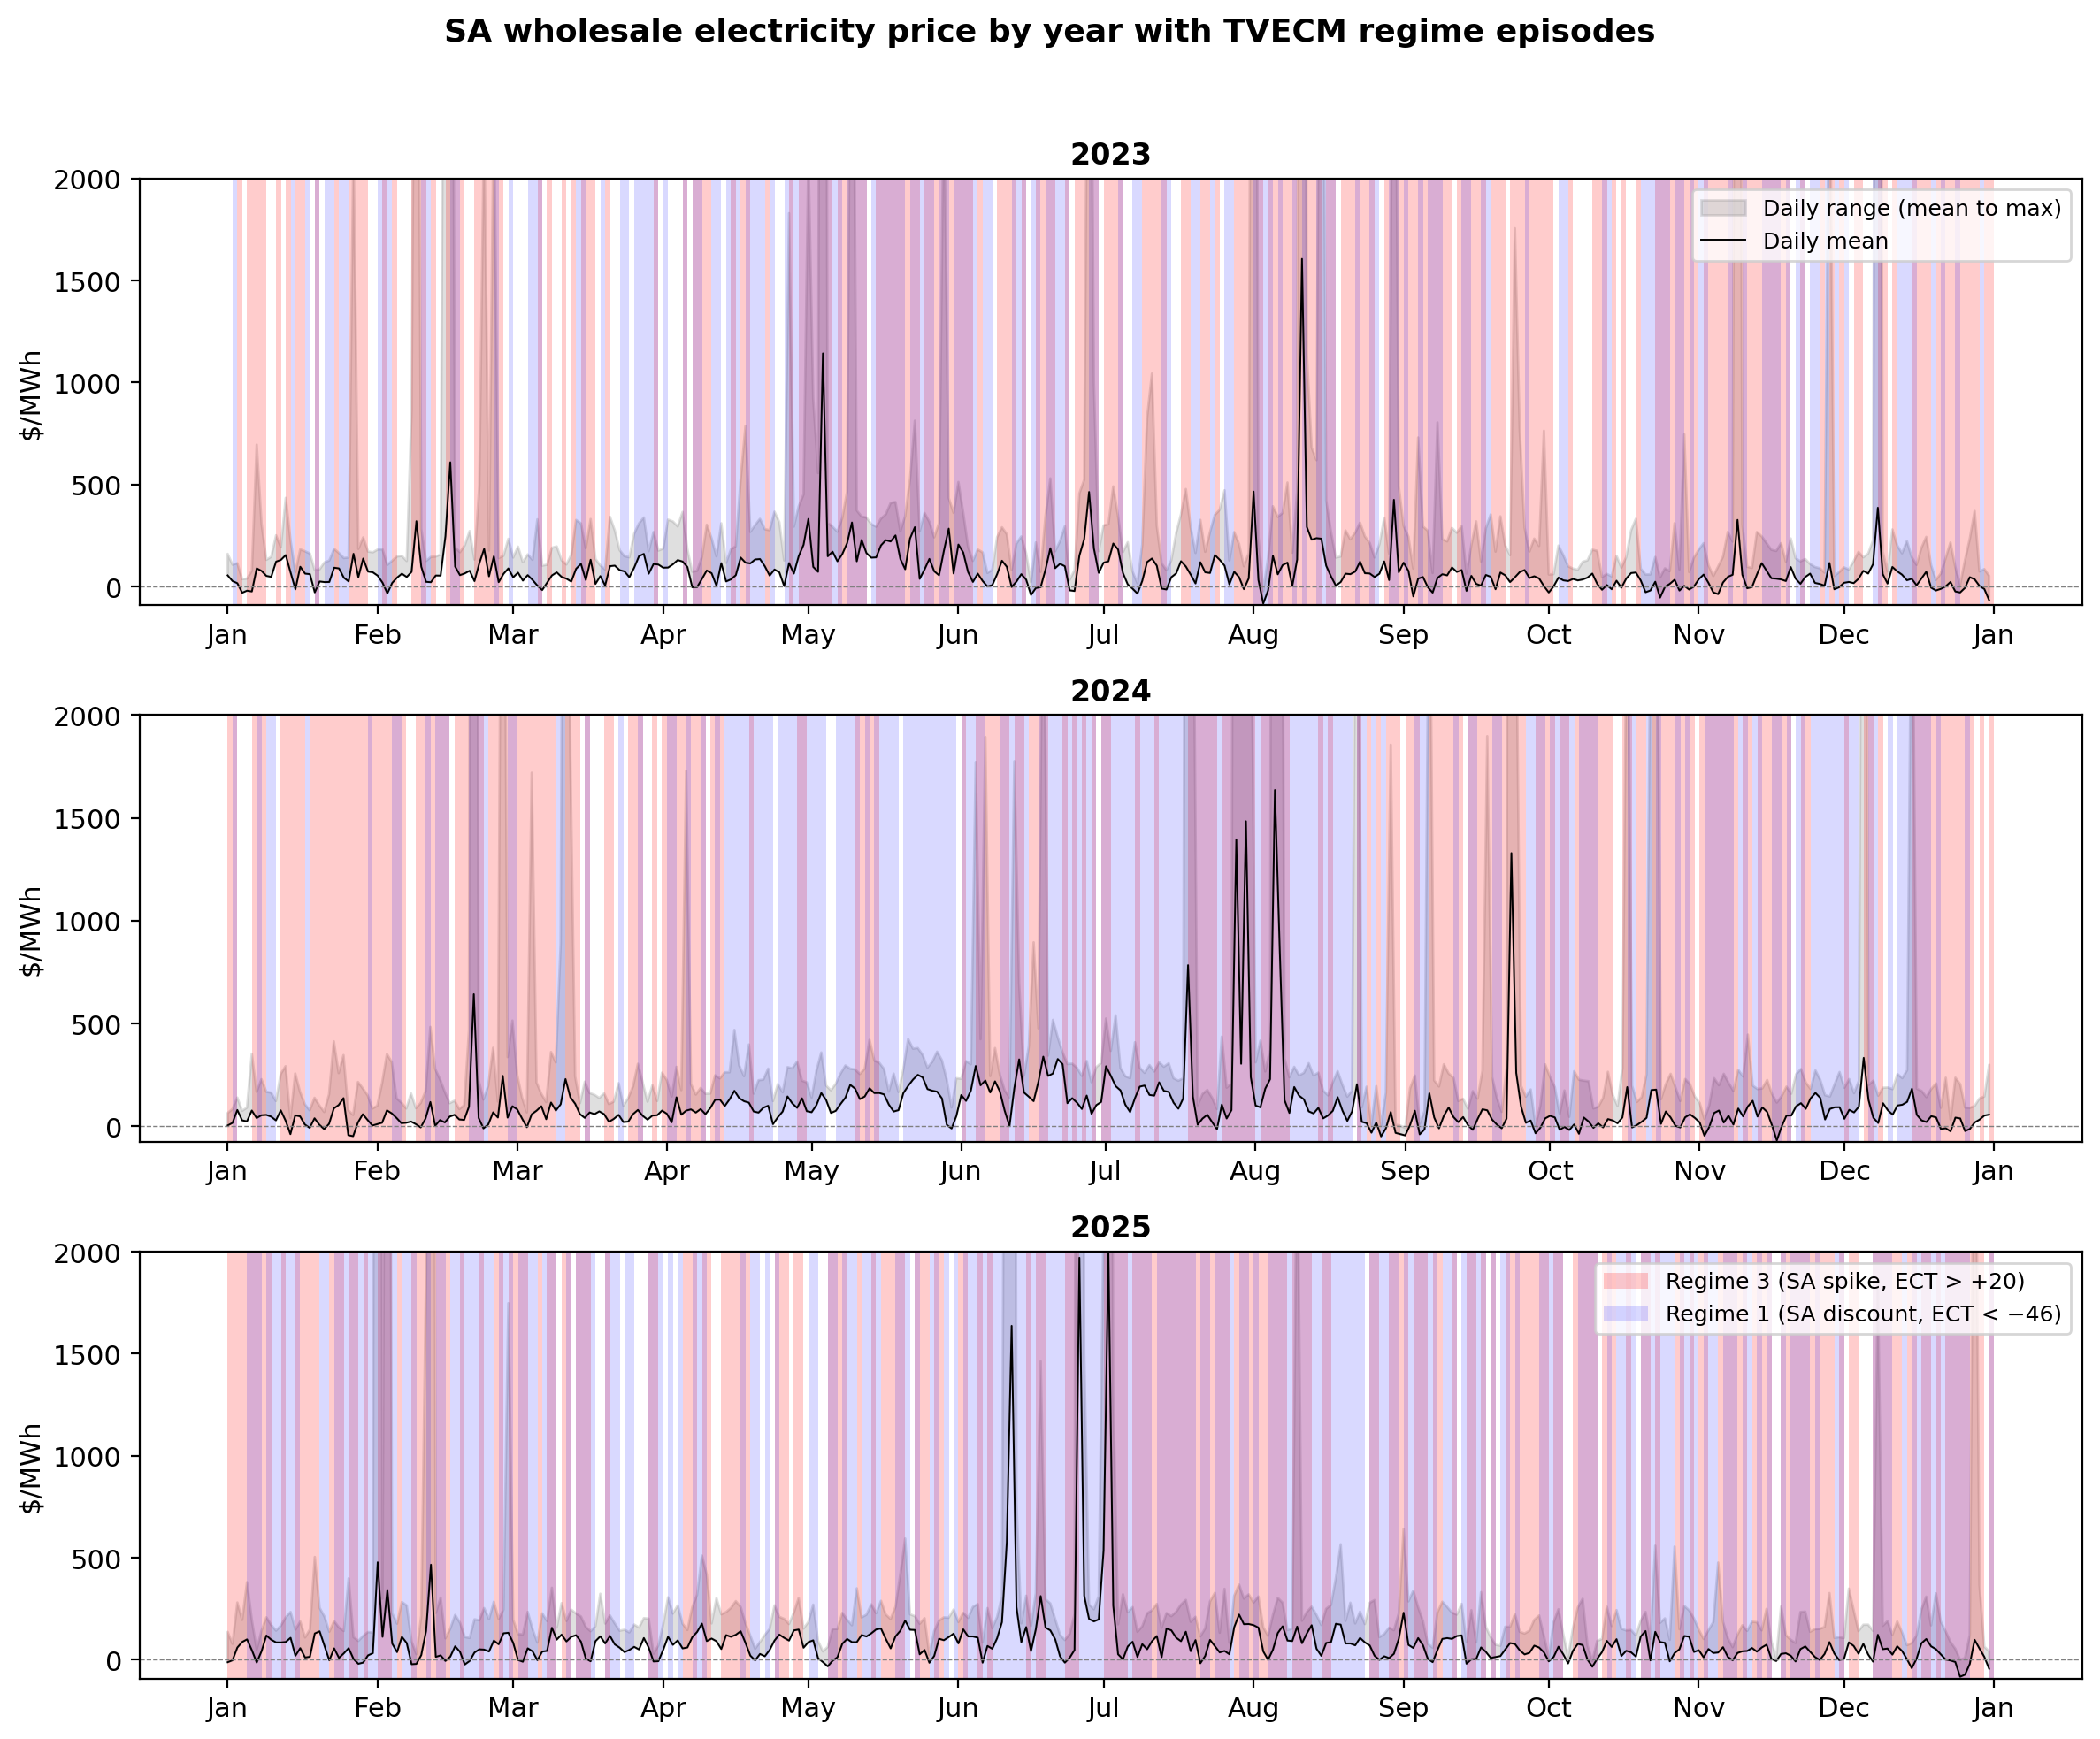
\includegraphics[width=\textwidth]{fig_sa_price_regimes.png}
  \caption{SA weekly mean wholesale price (2023--2025).  Red shading indicates
    weeks where more than 30\% of intervals fall in Regime~3 (spike).}
  \label{fig:price_regimes}
\end{figure}

\begin{figure}[htbp]
  \centering
  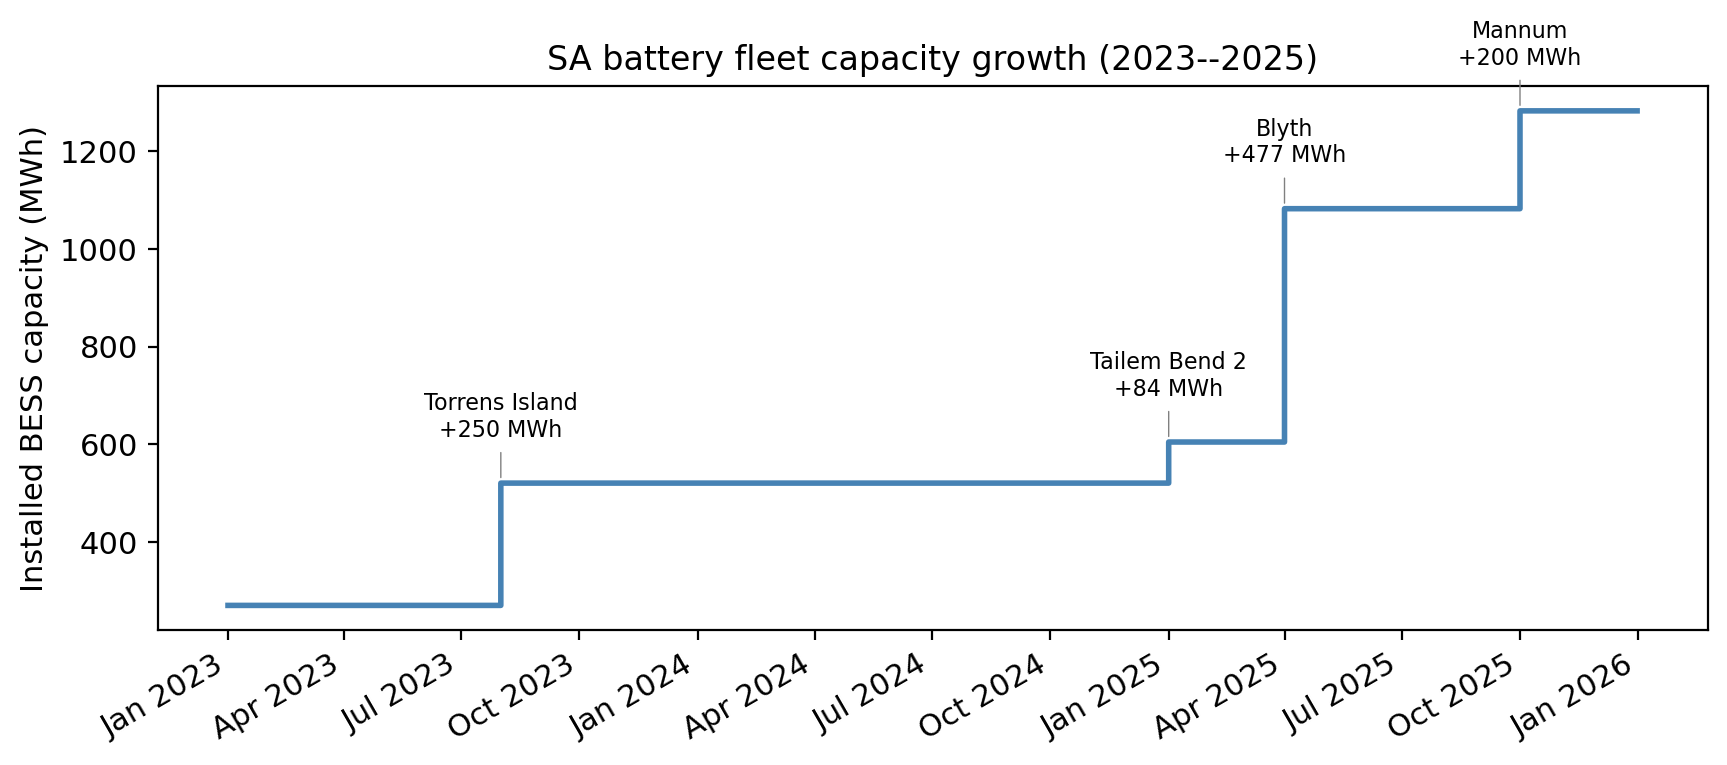
\includegraphics[width=\textwidth]{fig_capacity_growth.png}
  \caption{Step-function growth of SA installed BESS capacity (MWh).
    Annotations mark in-sample commissioning events used for the $Z^{newcap}$
    instrument.}
  \label{fig:capacity}
\end{figure}

\begin{figure}[htbp]
  \centering
  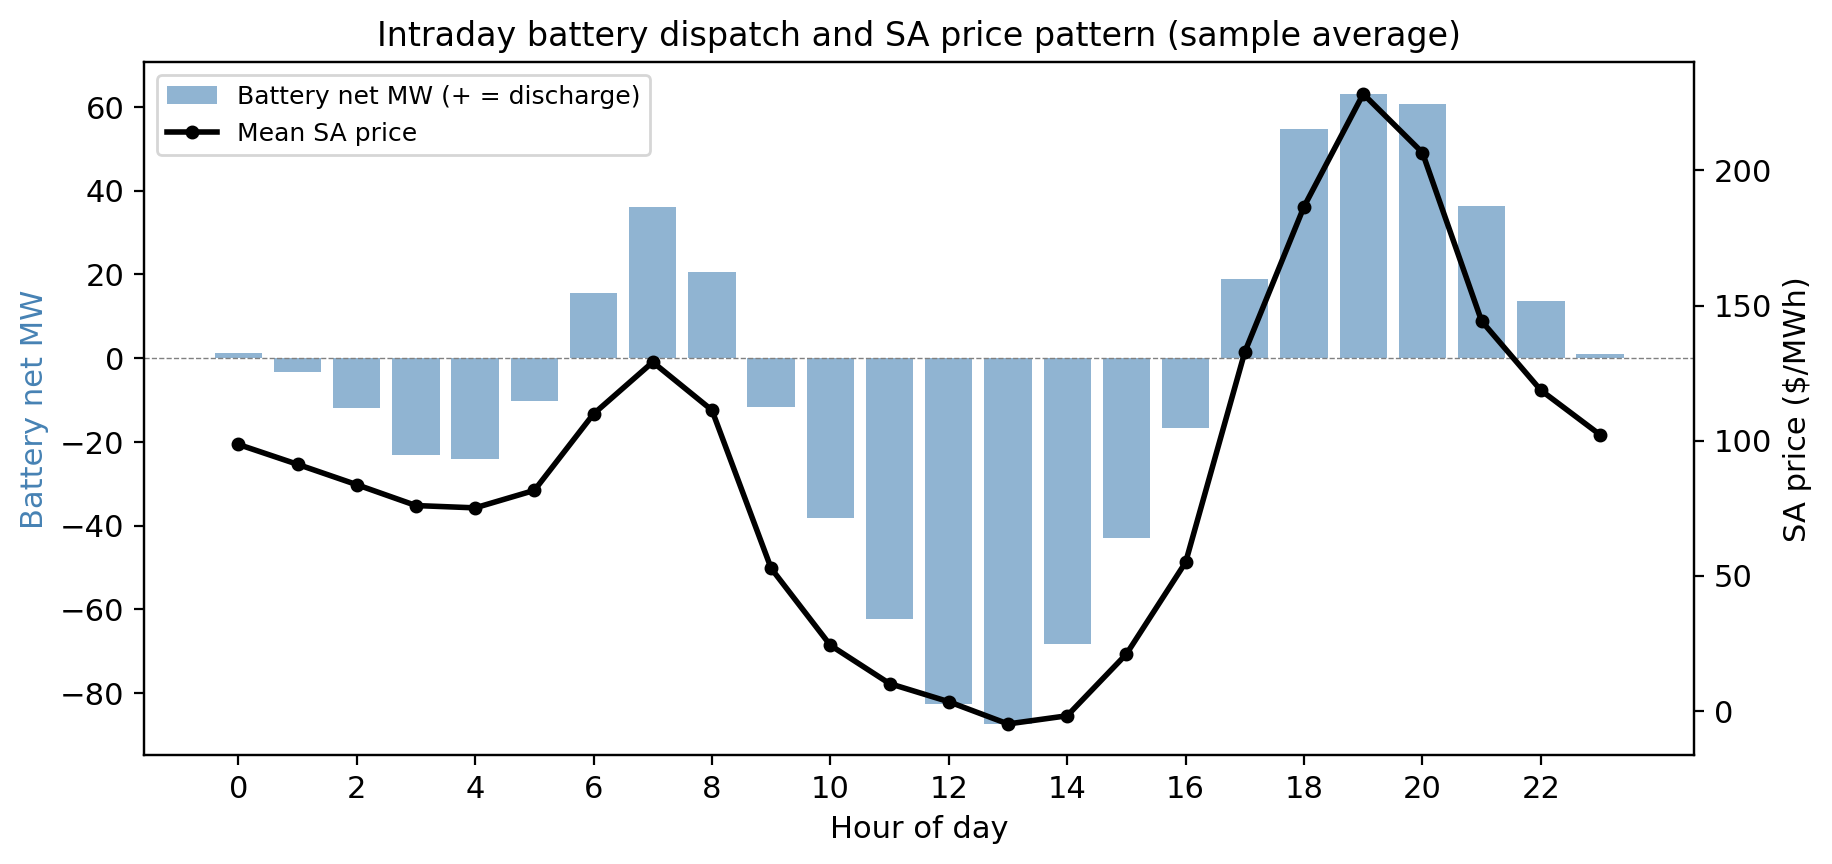
\includegraphics[width=\textwidth]{fig_intraday_pattern.png}
  \caption{Mean intraday battery net dispatch (bars) and SA spot price (line).
    Positive net MW indicates discharge; negative indicates charging.}
  \label{fig:intraday}
\end{figure}

\begin{figure}[htbp]
  \centering
  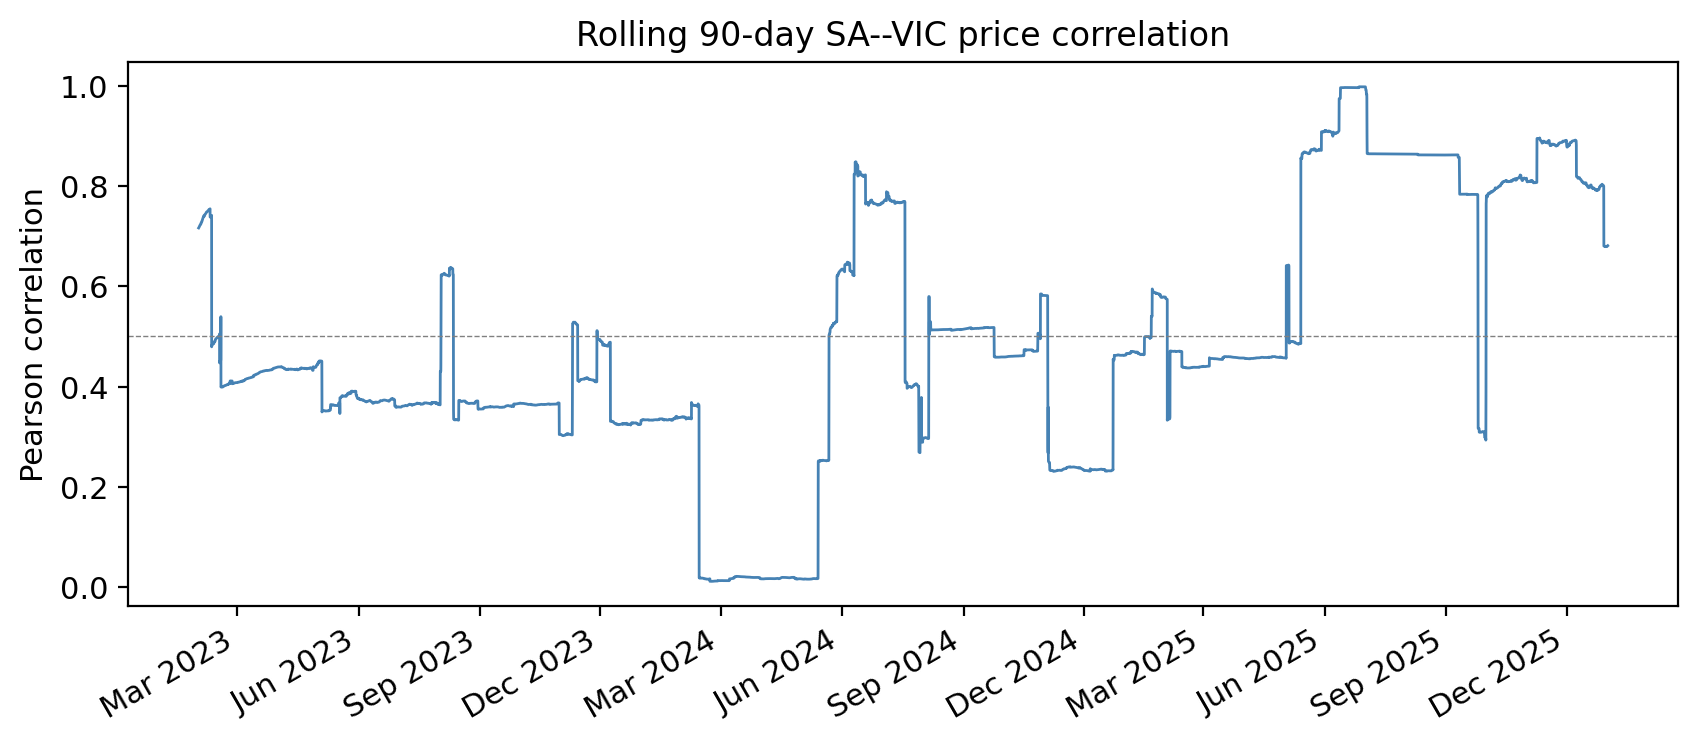
\includegraphics[width=\textwidth]{fig_rolling_correlation.png}
  \caption{Rolling 90-day Pearson correlation between SA and VIC wholesale
    prices.  The sharp increase from 2024 onward coincides with major BESS
    commissioning events.}
  \label{fig:correlation}
\end{figure}

%% ============================================================
\section{Econometric Methodology}
\label{sec:method}

\subsection{Pre-estimation Diagnostics}
\label{subsec:diagnostics}

\paragraph{Unit root tests.}
Table~\ref{tab:unitroot} reports ADF, Phillips--Perron (PP), and KPSS results.
ADF and PP both reject the unit root null in levels (ADF: $-22.51$ and $-20.86$
for SA and VIC; PP: $-98.87$ and $-79.99$), but these results warrant caution
for two reasons.  With $T = 52{,}608$, both tests accumulate power
against any departure from a pure random walk, including spot-market mean
reversion.  More directly, \textcite{escribano2011modelling} show that
additive spike outliers ``bias unit root inference towards rejection,''
since ADF-type tests assume homoskedastic, jump-free errors violated by the
spike distribution in Table~\ref{tab:desc}.
\textcite{weron2006modeling} similarly cautions against direct application of
standard unit root procedures to spike-prone electricity prices.

The KPSS test \parencite{kwiatkowski1992testing} complements this by reversing
the null: it tests level stationarity directly, so rejection is evidence
\textit{against} stationarity, and its variance-ratio construction is less
exposed to the outlier-inflation problem.  Both series yield KPSS statistics
exceeding the 1\% critical value in levels ($p = 0.010$), rejecting stationarity,
while first differences fall below the 10\% critical value ($p > 0.10$).  ADF
and PP confirm I(0) first differences ($p < 0.001$).  Both series are treated
as I(1); the mixed level evidence is consistent with the broader electricity
price literature \parencite{escribano2011modelling,weron2006modeling}.

\paragraph{Johansen cointegration.}
\textcite{johansen1988statistical} maximum-likelihood estimation of a four-lag VAR with a constant
restricted to the cointegrating space identifies one cointegrating vector
(Table~\ref{tab:johansen}).  The trace statistic of 8{,}739.4 and maximal
eigenvalue statistic of 4{,}811.2 vastly exceed their 5\% critical values of
15.49 and 14.26, though as with the unit root tests these figures are inflated
by spike heteroscedasticity.  Direct confirmation of cointegration is taken
instead from the ADF test on the estimated error-correction term: the statistic
of $-38.96$ ($p < 0.001$) confirms that
\begin{equation}
  \label{eq:ect}
  \ect_{t} = p_t^{SA} - 1.2103\, p_t^{VIC}
\end{equation}
is unambiguously stationary.  The cointegrating coefficient $\hat\beta = 1.2103$
reflects SA's structural tendency to trade at a slight premium to VIC,
consistent with the higher residual cost of the gas-peaking capacity that clears
the SA market during renewable shortfalls and the transmission costs embedded
in the Heywood interconnector.

\paragraph{Threshold selection.}
Three specifications are evaluated using the Hansen--Seo Rademacher wild
bootstrap (Table~\ref{tab:thresh}): a single threshold, a symmetric band, and a
two-threshold (three-regime) model.  All specifications include calendar dummy
controls (public holidays, weekends, and time-of-day buckets) as additional
regressors in the error-correction equation.  The two-threshold specification
wins decisively on every criterion: lowest bootstrap $p$-value ($p = 0.030$,
the only specification to reject linearity at the 5\% level), lowest AIC
(723{,}588 versus 725{,}273 for the symmetric band), lowest BIC, and highest
variance reduction.  The estimated thresholds, $\hat\gamma_L = -45.80$ and
$\hat\gamma_U = +20.02$\,\$/MWh, define an asymmetric no-arbitrage band that is
wider on the discount side.  This asymmetry is economically interpretable:
episodes of SA renewable oversupply are larger in magnitude and more persistent
than positive price spikes, consistent with the 27.5\% frequency of negative SA
prices observed in the data.  The ECT histogram (Figure~\ref{fig:ect}) confirms
that 80\% of observations fall within the band, with roughly 10\% in each tail.

\begin{figure}[htbp]
  \centering
  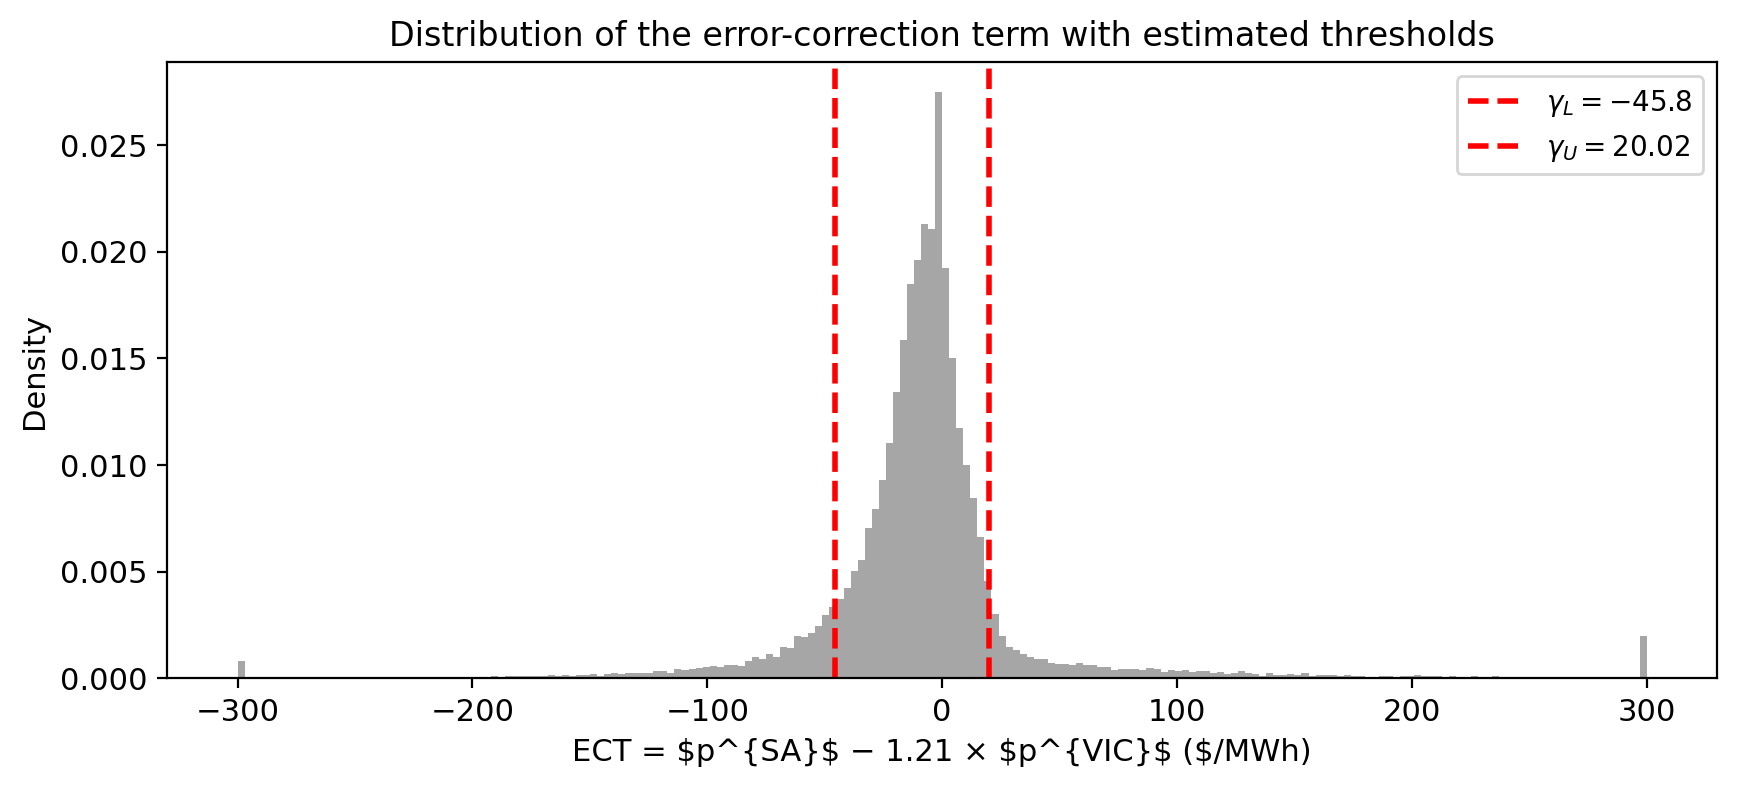
\includegraphics[width=\textwidth]{fig_ect_distribution.png}
  \caption{Histogram of $\ect_t = p_t^{SA} - 1.2103\,p_t^{VIC}$.  Dashed red
    lines mark the estimated thresholds $\hat\gamma_L = -45.80$ and
    $\hat\gamma_U = +20.02$\,\$/MWh.  The bulk of observations (80\%) fall
    within the no-arbitrage band (Regime~2).}
  \label{fig:ect}
\end{figure}

\subsection{Three-Regime TVECM}
\label{subsec:tvecm}

Regime membership is determined by the lagged $\ect_{t-1}$ relative to
$\hat\gamma_L$ and $\hat\gamma_U$:
\begin{equation}
  \label{eq:regime}
  r_t =
  \begin{cases}
    1 & \ect_{t-1} < -45.80 \quad (\text{SA deep discount, } N = 5{,}253) \\
    2 & -45.80 \le \ect_{t-1} \le +20.02 \quad (\text{no-arbitrage band, } N = 42{,}042) \\
    3 & \ect_{t-1} > +20.02 \quad (\text{SA price spike, } N = 5{,}257)
  \end{cases}
\end{equation}
Within each regime $r \in \{1,2,3\}$, OLS with Newey--West HAC standard errors
(12 lags) estimates:
\begin{equation}
  \label{eq:tvecm}
  \dsa_t = \mu_r + \alpha_r\,\ect_{t-1}
  + \sum_{i=1}^{4}\phi_i^r\,\dsa_{t-i}
  + \sum_{i=1}^{4}\psi_i^r\,\dvic_{t-i}
  + \beta_1^r B_t^{dis} + \beta_2^r B_t^{chg}
  + \boldsymbol{\delta}^{r\prime}\mathbf{x}_t + \varepsilon_t
\end{equation}
where $B_t^{dis}$ and $B_t^{chg}$ are battery discharge and charging (MW),
$\mathbf{x}_t$ collects wind generation, solar output, operational demand,
interconnector flows, and calendar dummy controls (public holidays, weekends,
and time-of-day buckets), and the same equation is estimated for $\dvic_t$.
Standard errors are Newey--West HAC \parencite{newey1987simple} with 12~lags;
full coefficient estimates appear in Table~\ref{tab:fullcoef}.
Lag order $L = 4$ is
AIC/BIC-optimal in the dominant Regime~2; lag robustness across
$L \in \{4,6,8,10,12\}$ confirms that key coefficients change by at most 0.04
(Table~\ref{tab:lagrobust}).

\subsection{Identification Strategy}
\label{subsec:identification}

Battery operators observe real-time prices and dispatch accordingly; contemporaneous
OLS therefore conflates the causal dampening effect with the reactive dispatch
channel, producing an upward-biased $\hat\beta_1^r$.  Three strategies address this.

\textbf{Predetermined regressors.}  Replacing $B_t^{dis}$ with $B_{t-1}^{dis}$
removes the contemporaneous simultaneity channel while preserving regime
heterogeneity.

\textbf{2SLS with capacity-normalised SOC.}  The primary instrument is
\begin{equation}
  \label{eq:soc}
  Z^{SOC}_{t-1} = \frac{\displaystyle\sum_{j=0}^{23}
    \bigl(B_{t-j}^{chg} - B_{t-j}^{dis}\bigr)\cdot 0.5\,\text{h}}{K_{t-1}}
\end{equation}
where $K_{t-1}$ is total installed BESS capacity (MWh) at $t-1$.  High lagged
SOC implies greater discharge headroom, creating a relevant first stage;
capacity normalisation removes the growing-fleet time trend that contaminates
unnormalised SOC (the Sargan $J$-test for raw MWh fails in Regime~2 at
$p < 0.001$).

\textbf{Commissioning-event instrument.}  $Z^{newcap}_{t-1}$ counts the total
MWh commissioned in the 14-day window ending at $t-1$.  Its exogeneity rests
on construction-contract timelines determined years in advance by project
finance decisions, not real-time market conditions.  Wu-Hausman and Sargan
over-identification tests \parencite{hausman1978specification,sargan1958estimation}
validate both instruments jointly (Table~\ref{tab:ivdiag}).

\subsection{Supplementary Robustness Models}
\label{subsec:supp}

Three supplementary models serve as robustness validators; estimates appear in
Section~\ref{subsec:robust} (GARCH-M: Table~\ref{tab:garch}) and
Appendix~A (Markov switching: Table~\ref{tab:msecm}; jump diffusion:
Table~\ref{tab:jumpdiff}).  A \textbf{GARCH(1,1)-$t$ extension}
\parencite{engle1982autoregressive,bollerslev1986generalized} verifies that OLS
coefficients are not invalidated by the IGARCH dynamics confirmed by Ljung-Box
tests on TVECM residuals.  A \textbf{three-state Markov-switching ECM}
\parencite{hamilton1989new}, estimated via the Baum--Welch EM algorithm,
provides an alternative regime classification that does not impose hard ECT
thresholds, testing whether the TVECM segmentation reflects genuine latent
states.  A \textbf{Merton-type jump-diffusion model} offers a continuous-time
complement, testing whether spike dynamics are consistent with a Poisson process
whose arrival rate declines as battery capacity grows.

%% ============================================================
\section{Results and Discussion}
\label{sec:results}

\subsection{Error-Correction Asymmetry}
\label{subsec:eca}

Table~\ref{tab:alpha} reports the error-correction speeds $\alpha_r$; the Wald
test strongly rejects equality across regimes ($F(2) = 29.96$, $p < 0.001$),
validating the three-regime TVECM against a linear VECM.

In \textbf{Regime~3} (SA price spike), only the SA equation exhibits a
significant adjustment: $\hat\alpha_{SA} = -0.349$ ($p < 0.001$), implying a
half-life of approximately 0.8~hours.  The VIC adjustment speed is
indistinguishable from zero ($\hat\alpha_{VIC} = -0.002$, $p = 0.14$).  The
economic mechanism is directional: when SA prices spike above the no-arbitrage
ceiling identified in Section~\ref{subsec:diagnostics}, VIC imports via the
Heywood interconnector suppress the SA premium without triggering any
VIC-side price formation response.

In \textbf{Regime~1} (SA deep discount), the pattern reverses: VIC corrects
alone ($\hat\alpha_{VIC} = +0.525^{***}$), falling toward the level implied by
cheap SA renewable exports, while SA is statistically insignificant
($\hat\alpha_{SA} = +0.213$, $p = 0.18$).  SA generators operating at capacity
during renewable surplus cannot further reduce output, so the correction occurs
entirely on the VIC side.  This price-leadership asymmetry is the empirical
signature of the band-of-inaction model \parencite{balke1997threshold}: error
correction is regime-specific, directional, and only triggered once the spread
crosses the transaction-cost thresholds established in the diagnostics.

Impulse-response functions (Figure~\ref{fig:irf}; Table~\ref{tab:irfdata}) make
this asymmetry visually transparent.  A 1~MW battery discharge shock dissipates
almost entirely within six 30-minute periods in Regime~3 (cumulative SA price at
$h = 12$: $+0.026$\,\$/MWh, down from the initial impact of $+1.20$\,\$/MWh),
driven by the strong negative $\hat\alpha_{SA}$.  In Regime~1, the identical
shock persists at $+0.268$\,\$/MWh after six hours because the insignificant
$\hat\alpha_{SA}$ generates no restoring force.  The VIC response in the spike
regime is negligible ($+0.010$\,\$/MWh at $h = 12$), confirming that the
battery-price channel is SA-local.

\begin{figure}[htbp]
  \centering
  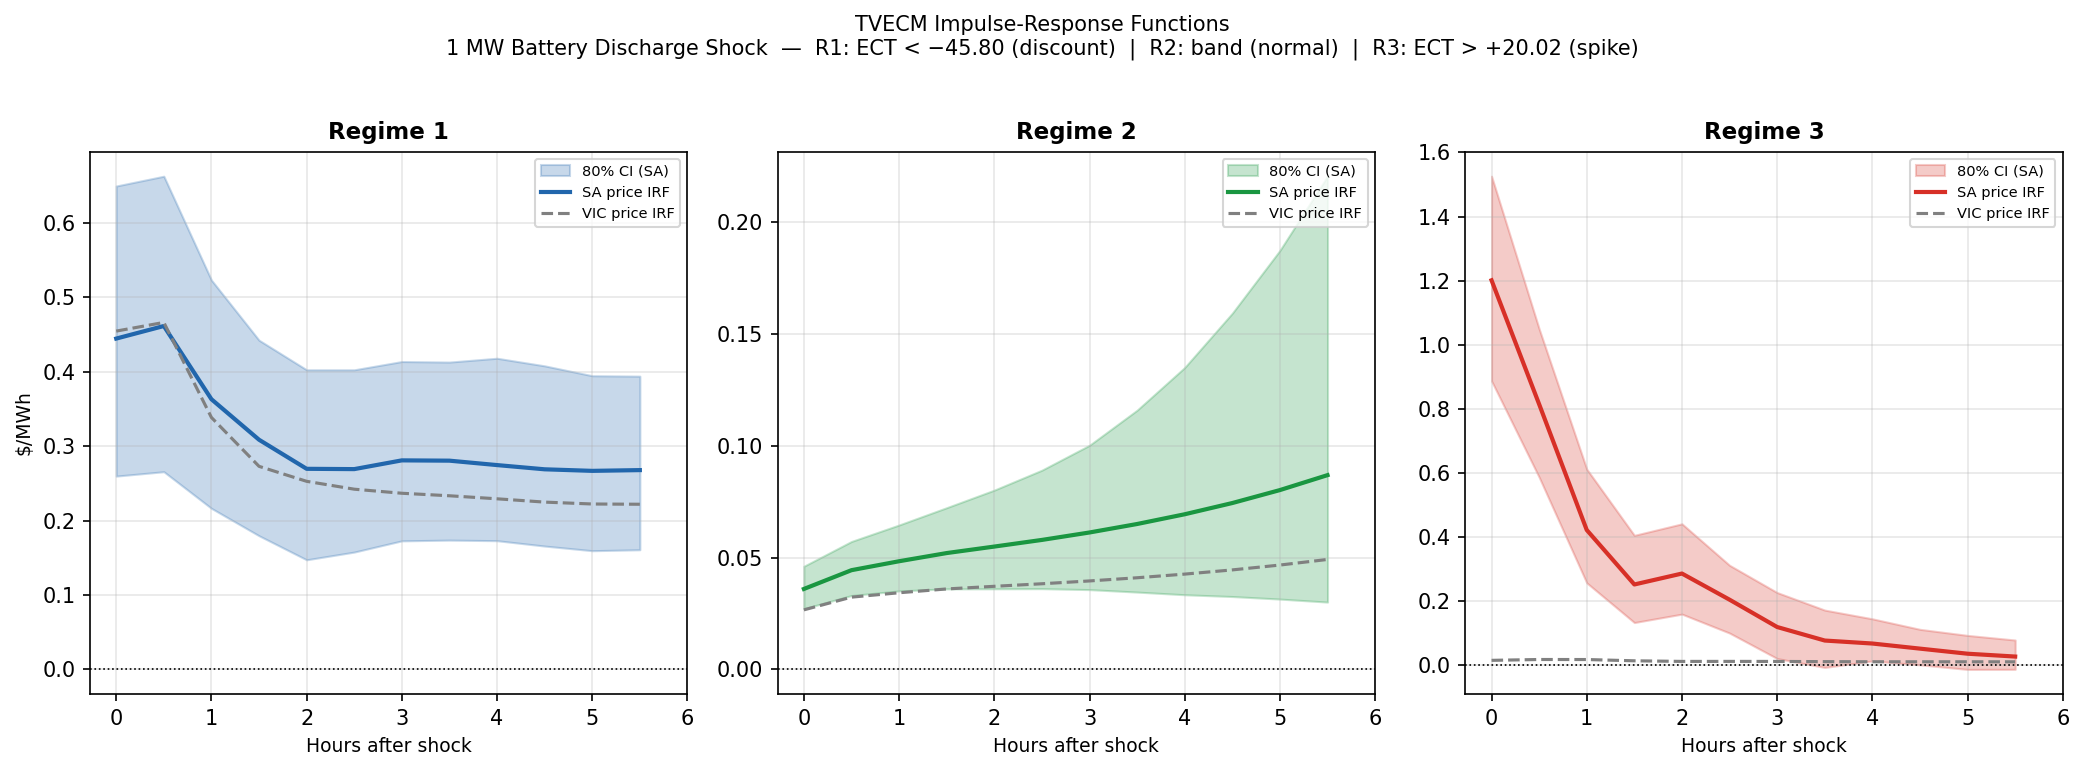
\includegraphics[width=\textwidth]{phase8_irf.png}
  \caption{Regime-conditional impulse-response functions for a 1~MW battery
    discharge shock.  Solid lines: SA price level (cumulative); dashed lines:
    VIC price level.  Shaded bands: 80\% wild bootstrap confidence interval
    (Rademacher, $N = 500$).  Horizontal dotted lines at zero.}
  \label{fig:irf}
\end{figure}

\begin{table}[htbp]
  \centering
  \caption{Error-correction speeds by regime and equation}
  \label{tab:alpha}
  \begin{threeparttable}
    \begin{tabular}{lC{2.2cm}C{2.2cm}C{2.2cm}C{2.4cm}}
      \toprule
      & Regime 1 & Regime 2 & Regime 3 & Wald $F(2)$ \\
      & (discount) & (band) & (spike) & \\
      \midrule
      SA equation: $\hat\alpha_{SA}$
        & $+0.213$ & $+0.249^{***}$ & $-0.349^{***}$ & \\
        & $(0.160)$ & $(0.056)$      & $(0.055)$      & \\[3pt]
      VIC equation: $\hat\alpha_{VIC}$
        & $+0.525^{***}$ & $+0.082^{***}$ & $-0.002$ & \\
        & $(0.138)$      & $(0.011)$      & $(0.001)$ & \\[3pt]
      \midrule
      Wald test ($\alpha$ equal across regimes): & & & & $29.96^{***}$ \\
      Half-life (SA, spike regime): & & & 0.8 h & \\
      $N$ & 5,253 & 42,042 & 5,257 & \\
      \bottomrule
    \end{tabular}
    \begin{tablenotes}
      \small
      \item \textit{Note:} HAC standard errors (Newey--West, 12 lags) in parentheses.
        Half-life $= -\ln 2 \,/\, \ln(1 + \hat\alpha_{SA})$.
        $^{***}p<0.01$, $^{**}p<0.05$, $^{*}p<0.10$.
    \end{tablenotes}
  \end{threeparttable}
\end{table}

\subsection{Identification of the Causal Battery Effect}
\label{subsec:battery}

Table~\ref{tab:batteries} presents $\hat\beta_1^r$ across the three
identification strategies.  The na\"ive OLS estimates are uniformly positive
across all regimes, a textbook simultaneity bias: batteries discharge
\textit{in response to} high prices, generating a positive empirical correlation
that reverses the true causal direction.  The Wald test confirms that these
coefficients are significantly regime-dependent ($F(2) = 8.19$, $p < 0.001$),
so the bias itself is regime-specific.

The contrast is most instructive in \textbf{Regime~3} (spike).  The
contemporaneous OLS estimate ($+1.201^{***}$) is dominated by reactive dispatch.
Replacing the contemporaneous regressor with its one-period lag removes this
channel and reverses the sign ($-0.194$, $n.s.$), consistent with a causal
dampening effect that is directionally correct but statistically imprecise at the
individual-period level given the extreme residual noise
($\hat\sigma_\varepsilon \approx \$589$/MWh in Regime~3).  Crucially, the
Wu-Hausman test fails to reject exogeneity in Regime~3 ($p = 0.731$), likely
reflecting low power against this extreme residual variance rather than genuine
exogeneity of battery dispatch during price spikes.  Since 2SLS is not warranted
when endogeneity cannot be established, the \textbf{lagged OLS estimate}
($-0.194$, $n.s.$) is the preferred estimator for Regime~3: it removes
contemporaneous simultaneity by construction without requiring an instrument
validity assumption.  In Regimes~1 and~2, where Wu-Hausman confirms endogeneity
($p = 0.001$ and $p < 0.001$ respectively), 2SLS remains the appropriate
estimator.  The lagged OLS estimate ($-0.194$, $s.e.=0.173$, 95\% CI
$[-0.53,\;+0.15]$) cannot exclude zero but is consistent with a small marginal
effect: once peaking generators set the marginal price, additional battery
output cannot meaningfully compress the clearing price
\parencite{joskow2011comparing}.  This interpretation does not rest on the
lagged OLS coefficient alone; it is corroborated by the capacity-interaction
model (the spike-regime marginal effect
converges to $+0.29$, $n.s.$, by December~2025; Table~\ref{tab:interact}) and
by rolling-window threshold analysis showing a monotonic decline in spike-regime
frequency from 9.4\% to 5.0\%.  Together, these results indicate that the
primary welfare channel operates through spike \textit{prevention}: batteries
are strategically pre-positioned to displace peaker dispatch entirely, rather
than through compression of spikes already underway.

Table~\ref{tab:ivdiag} reports IV diagnostics.  \textbf{First-stage relevance:}
partial $F$-statistics for $Z^{SOC}$ exceed the \textcite{staiger1997instrumental}
threshold of 10 in all regimes (52.3 in Regime~1; 198.2 in Regime~2; 30.2 in
Regime~3).  \textbf{Endogeneity:} Wu-Hausman tests confirm endogeneity at 1\% in
Regimes~1 and~2, justifying 2SLS in those regimes.  The test fails to reject
exogeneity in Regime~3 ($p = 0.731$); given the extreme residual noise in the
spike regime, this likely reflects insufficient power rather than genuine
exogeneity, but it means that 2SLS is not statistically warranted there.  We
therefore adopt the lagged OLS estimate as the primary Regime~3 result
(Table~\ref{tab:batteries}).  \textbf{Instrument validity:} the Sargan $J$-test
for the over-identified specification with $Z^{SOC}$ and $Z^{newcap}$ jointly
yields $p = 0.164$ in Regime~2 and $p > 0.68$ in the outer regimes, validating
the SOC exclusion restriction in the regimes where 2SLS is applied.  By
contrast, the raw-MWh SOC instrument fails the Sargan test in Regime~2
($p < 0.001$), confirming that capacity normalisation is essential to remove
the growing-fleet trend contamination.

\begin{table}[htbp]
  \centering
  \caption{Battery discharge coefficient across three identification strategies
    (SA equation)}
  \label{tab:batteries}
  \begin{threeparttable}
    \begin{tabular}{lC{3cm}C{3cm}C{3cm}}
      \toprule
      Regime & OLS & Lagged OLS & 2SLS \\
      \midrule
      1 (discount)
        & $+0.445^{***}$ & $+0.003$ & $+1.774^{***}$ \\
        & $(0.151)$      & $(0.039)$ & $(0.208)$ \\[3pt]
      2 (band)
        & $+0.036^{***}$ & $-0.029$ & $+0.428^{***}$ \\
        & $(0.008)$      & $(0.022)$ & $(0.022)$ \\[3pt]
      3 (spike)
        & $+1.201^{***}$ & $-0.194$ & $+0.776^{**}$ \\
        & $(0.386)$      & $(0.173)$ & $(0.369)$ \\
      \midrule
      Wald $F(2)$ on $\beta_{dis}$ & $8.19^{***}$ & 0.16 & — \\
      \bottomrule
    \end{tabular}
    \begin{tablenotes}
      \small
      \item \textit{Note:} HAC standard errors (Newey--West, 12 lags) in
        parentheses.  Lagged OLS uses $B_{t-1}^{dis}$; 2SLS instruments with
        $Z^{SOC}_{t-1}$.  Wald $F(2)$ tests equal coefficients across regimes.
        $^{***}p<0.01$, $^{**}p<0.05$, $^{*}p<0.10$.
    \end{tablenotes}
  \end{threeparttable}
\end{table}

\begin{table}[htbp]
  \centering
  \caption{Instrumental variable diagnostics by regime}
  \label{tab:ivdiag}
  \begin{threeparttable}
    \begin{tabular}{lC{2.6cm}C{2.6cm}C{2.6cm}}
      \toprule
      Diagnostic & Regime 1 & Regime 2 & Regime 3 \\
      \midrule
      First-stage $F$ ($Z^{SOC}$) & 52.30 & 198.22 & 30.20 \\
      Wu-Hausman $p$-value & $0.001^{***}$ & $<0.001^{***}$ & 0.731 \\[4pt]
      \multicolumn{4}{l}{\textit{Sargan $p$-value (Model A: $Z^{SOC}$ + $Z^{raw}$)}} \\
      & $0.086^{*}$ & $<0.001^{***}$ & 0.319 \\[4pt]
      \multicolumn{4}{l}{\textit{Sargan $p$-value (Model B: $Z^{SOC}$ + $Z^{newcap}$)}} \\
      & 0.689 & \textbf{0.164} & 0.711 \\
      \bottomrule
    \end{tabular}
    \begin{tablenotes}
      \small
      \item \textit{Note:} $Z^{SOC}$ = capacity-normalised 12-hour rolling SOC
        (lagged~1); $Z^{raw}$ = unnormalised raw MWh SOC (lagged~1); $Z^{newcap}$
        = BESS commissioned in preceding 14-day window (lagged~1, four in-sample
        commissioning events).  Sargan df\,=\,1 (one over-identifying restriction).
        Model A fails in Regime~2 because raw MWh SOC carries a growing-fleet
        trend; Model B passes in all regimes.
        $^{***}p<0.01$, $^{*}p<0.10$.
    \end{tablenotes}
  \end{threeparttable}
\end{table}

\subsection{Robustness and Fleet Maturation}
\label{subsec:robust}

\paragraph{GARCH-M robustness.}
Ljung-Box tests on TVECM residuals yield $p \approx 0.000$ in Regimes~1 and 3
at all lag orders up to $L = 12$ (Table~\ref{tab:lagrobust}), confirming that
the autocorrelation reflects conditional heteroscedasticity rather than
mean-equation mis-specification.  The GARCH(1,1)-$t$ estimates
(Table~\ref{tab:garch}) reveal integrated variance in Regimes~2 and 3
($\hat\alpha_G + \hat\beta_G = 1.0$, IGARCH) and very heavy tails
($\hat\nu \approx 2.9$) across all regimes, consistent with
\textcite{weron2006modeling} and \textcite{escribano2011modelling}.  The central
finding is that battery-discharge coefficients change by at most 0.027 across
regimes after GARCH-M augmentation, with significance levels preserved.  This
confirms that baseline OLS and 2SLS estimates are robust to IGARCH dynamics:
coefficient levels are unaffected ($\Delta\hat\beta_{dis} < 0.027$), and
inference is already addressed by the HAC bandwidth.

\paragraph{Markov-switching validation.}
A three-state Markov-switching ECM \parencite{hamilton1989new}, estimated via
the Baum--Welch EM algorithm, provides an alternative regime classification
that does not impose hard ECT thresholds.  Because the two models classify on
fundamentally different dimensions --- the TVECM partitions by the ECT level
(price \textit{spread}), while the MS-ECM partitions by conditional volatility
--- direct label concordance is low (32.1\% overall;
Table~\ref{tab:msecm}, Panel~C), and a close one-to-one mapping should not be
expected.  The validation instead comes from the structural parameters: the
MS-ECM's high-volatility state (S3, $\hat\sigma = 1{,}819$) recovers an
error-correction speed of $\hat\alpha = -0.352^{***}$, nearly identical to the
TVECM spike-regime estimate ($\hat\alpha_{SA} = -0.349^{***}$), while its
low-volatility state (S1) yields a near-zero $\hat\alpha$, mirroring the
insignificant TVECM discount-regime adjustment.  The two models thus
independently identify qualitatively similar dynamics --- fast mean-reversion
in extreme states, near-zero adjustment in calm states --- even though they
segment the sample by different criteria.

\paragraph{Jump-diffusion complement.}
A Merton-type jump-diffusion model decomposes SA price changes into a continuous
diffusion component and a Poisson jump process \parencite{merton1976option}, estimated
by maximum likelihood (Table~\ref{tab:jumpdiff}).  The jump mean is
\$368/MWh with standard deviation \$1{,}359/MWh; the average jump probability is
3.7\% per interval, versus the 10.0\% TVECM Regime~3 share, consistent with R3
encompassing moderate spike episodes that fall below the mixture jump threshold.
Battery discharge enters through two channels: a direct drift coefficient
$\hat\beta_{dis} = -0.054^{***}$ (price dampening) and a positive intensity
coefficient $\hat\lambda_{dis} = +0.005^{***}$, indicating that operators increase
discharge ahead of anticipated extreme events.  The model improves AIC by 213{,}849
relative to the OLS baseline, confirming that tail dynamics require explicit
mixture modelling.

\paragraph{Fleet maturation.}
A capacity-interaction term tests whether the battery-price relationship
changed as the fleet grew.  The interaction $\hat\gamma_{dis}$ is negative and significant in Regimes~2
and 3 ($p = 0.001$); the spike-regime marginal effect fell from $+4.76^{***}$
(271~MWh, January 2023) to $+0.29$ (n.s., December 2025), a 94\% reduction
(Table~\ref{tab:interact}).  In the band regime the decline is
even more complete: from $+0.155^{***}$ to $-0.007$ (n.s., December 2025).
Because the end-of-sample OLS marginal effect is indistinguishable from zero in
both regimes while the lagged OLS causal estimate remains at $-0.19$, this
trajectory is best interpreted as the progressive elimination of the reactive-dispatch
simultaneity component as the fleet matures toward strategic pre-positioning.

Rolling-window threshold analysis corroborates the welfare story: spike-regime
frequency fell monotonically from 9.4\% (2023) to 7.2\% (2024) to 5.0\% (2025),
consistent with an expanding fleet preventing spike events from materialising
at all.  Figure~\ref{fig:aug_comparison} illustrates the spike-prevention channel
directly: August 2023 recorded 24.5\% of intervals in the spike regime with a
maximum price of \$11{,}057/MWh and 112 intervals above \$300/MWh; August 2025,
with 2.4$\times$ the installed capacity, recorded 8.7\%, \$2{,}734/MWh, and
just 19 such intervals, representing an 83\% reduction.

\begin{figure}[htbp]
  \centering
  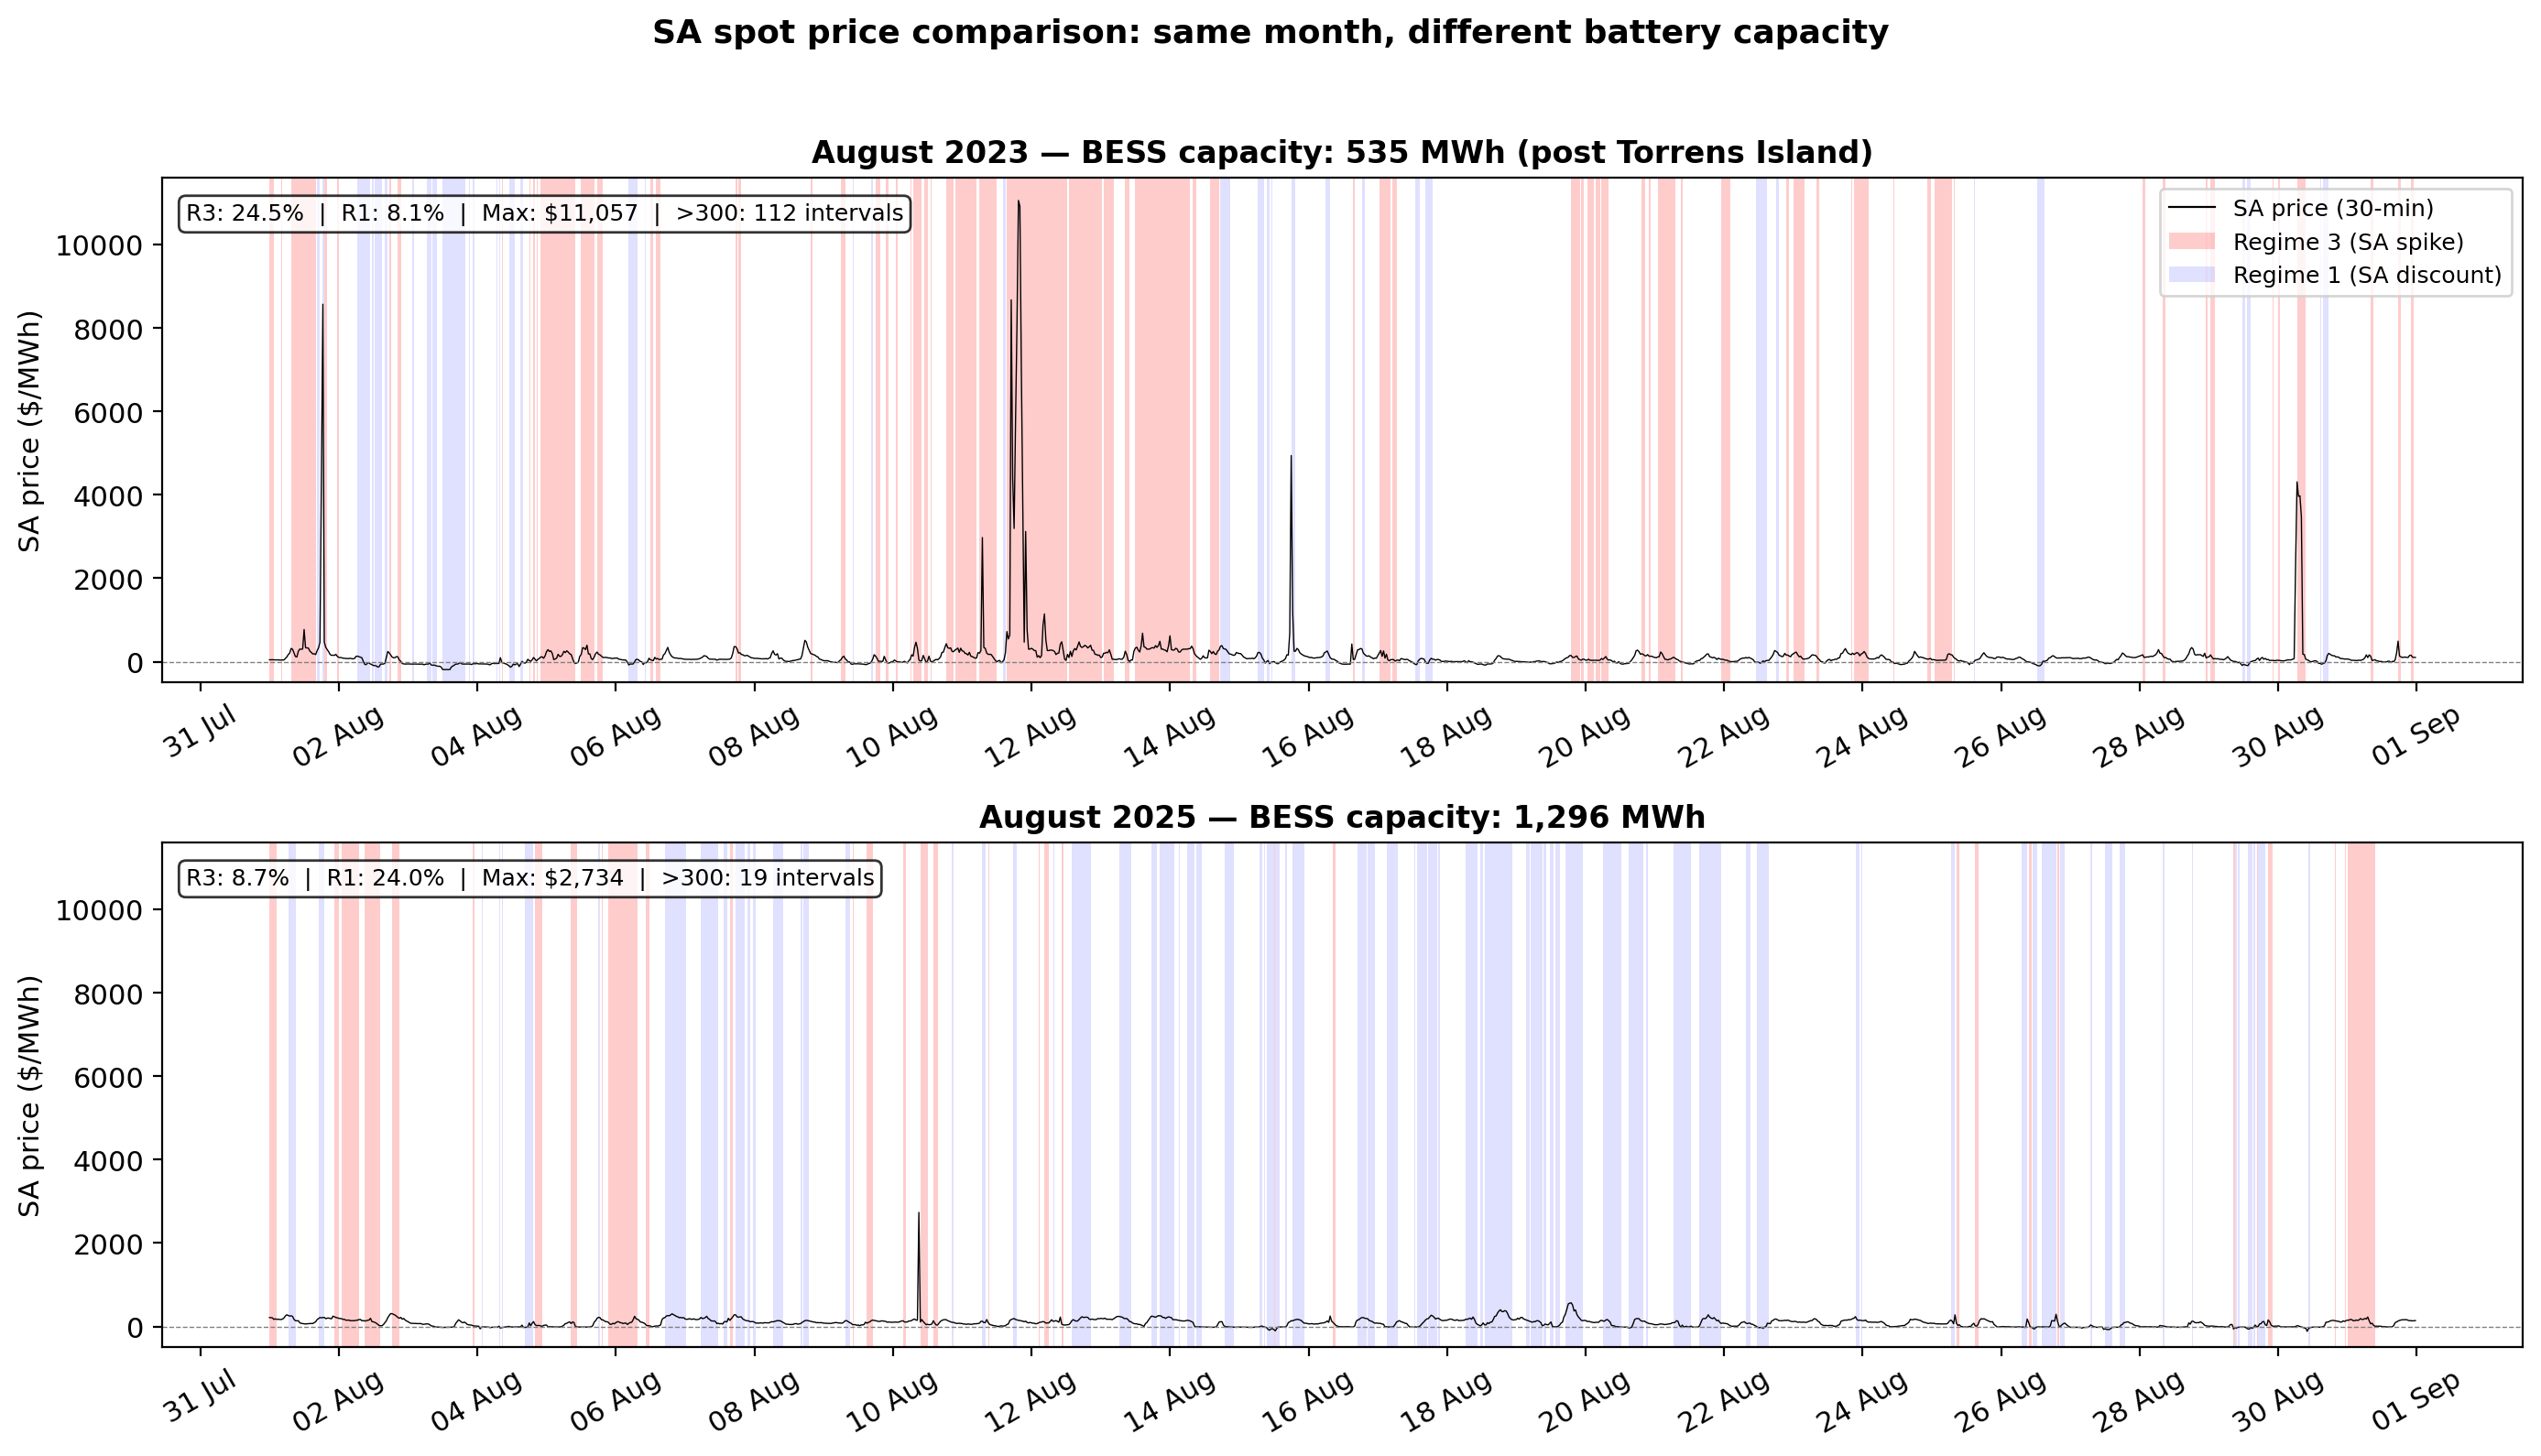
\includegraphics[width=\textwidth]{fig_aug_comparison.png}
  \caption{SA spot price at 30-minute resolution for August 2023 (top) and
    August 2025 (bottom).  Red shading: Regime~3 (spike, $\ect_{t-1} > +20$);
    blue shading: Regime~1 (discount, $\ect_{t-1} < -46$).  Annotation boxes
    report regime shares, maximum price, and count of intervals above \$300/MWh.
    Both panels share the same vertical axis.}
  \label{fig:aug_comparison}
\end{figure}

\begin{table}[htbp]
  \centering
  \caption{GARCH(1,1)-$t$ parameters and battery coefficient robustness}
  \label{tab:garch}
  \begin{threeparttable}
    \begin{tabular}{lC{2.4cm}C{2.4cm}C{2.4cm}}
      \toprule
      Parameter & Regime 1 & Regime 2 & Regime 3 \\
      \midrule
      $\hat\alpha_G$ (ARCH) & $0.841^{***}$ & $0.662^{***}$ & $0.856^{***}$ \\
      $\hat\beta_G$ (GARCH) & $0.114^{***}$ & $0.338^{***}$ & $0.144^{***}$ \\
      $\hat\alpha_G + \hat\beta_G$ & 0.954 & \textbf{1.000 (IGARCH)} & \textbf{1.000 (IGARCH)} \\
      $\hat\nu$ (Student-$t$ d.o.f.) & 3.01 & 2.86 & 2.82 \\
      $\hat\delta_r$ (risk premium) & $-1.957^{*}$ & $-0.004$ & $-0.850$ \\
      \midrule
      $\hat\beta_{dis}$: OLS baseline & $+0.445$ & $+0.036$ & $+1.201$ \\
      $\hat\beta_{dis}$: GARCH-M & $+0.443$ & $+0.036$ & $+1.228$ \\
      Change & $-0.001$ & $<0.001$ & $+0.027$ \\
      \bottomrule
    \end{tabular}
    \begin{tablenotes}
      \small
      \item \textit{Note:} Convergence in $\leq 9$ iterations.  Risk premium
        $\delta_r$ is the coefficient on $\hat\sigma_t$ in the mean equation.
        $^{***}p<0.01$, $^{*}p<0.10$.
    \end{tablenotes}
  \end{threeparttable}
\end{table}

\begin{table}[htbp]
  \centering
  \caption{Capacity-interaction model: predicted marginal effects
    $\partial\dsa/\partial B^{dis}$ (SA equation)}
  \label{tab:interact}
  \begin{threeparttable}
    \begin{tabular}{lC{2.0cm}C{2.4cm}C{2.4cm}C{2.4cm}}
      \toprule
      Regime & $\hat\gamma_{dis}$ & Jan 2023 & Jan 2024 & Dec 2025 \\
      & & (271~MWh) & (521~MWh) & (1{,}282~MWh) \\
      \midrule
      1 & $-0.265$ & $+0.762^{**}$ & $+0.658^{***}$ & $+0.342^{*}$ \\
        & $(0.230)$ & $(0.298)$ & $(0.224)$ & $(0.183)$ \\[3pt]
      2 & $-0.102^{***}$ & $+0.155^{***}$ & $+0.115^{***}$ & $-0.007$ \\
        & $(0.030)$ & $(0.040)$ & $(0.029)$ & $(0.011)$ \\[3pt]
      3 & $-2.819^{***}$ & $+4.763^{***}$ & $+3.657^{***}$ & $+0.288$ \\
        & $(0.876)$ & $(1.308)$ & $(0.978)$ & $(0.338)$ \\
      \bottomrule
    \end{tabular}
    \begin{tablenotes}
      \small
      \item \textit{Note:} $\hat\gamma_{dis}$ is the coefficient on
        $B_t^{dis} \times cap\_norm_t$.  Predicted marginals
        $\hat\beta_{dis}^r + \hat\gamma_{dis}^r \times cap\_norm$ at stated
        capacity levels, with delta-method standard errors.
        $\bar{K} = 636.9$~MWh.
        $^{***}p<0.01$, $^{**}p<0.05$, $^{*}p<0.10$.
    \end{tablenotes}
  \end{threeparttable}
\end{table}

%% ============================================================
\section{Conclusion and Limitations}
\label{sec:conclusion}

The main finding is that growing battery storage lowers SA wholesale electricity
prices primarily through a preventive channel.  The BESS fleet's 4.7-fold
expansion from 2023 to 2025 was accompanied by a monotonic decline in
spike-regime frequency from 9.4\% to 5.0\% and an 83\% reduction in high-price
intervals between August 2023 and August 2025.  The causal within-episode dampening effect appears small once price spikes have
already materialised: the predetermined-regressor estimate in the spike regime
($-0.19$, $n.s.$) --- the preferred estimator given that the Wu-Hausman test
does not warrant 2SLS there --- resolves the simultaneity bias that inflates
the raw OLS coefficient ($+1.20^{***}$), though the wide confidence interval
precludes a precise conclusion.  The capacity-interaction model and declining
spike-regime frequency corroborate this interpretation, jointly indicating that
the fleet's welfare contribution operates primarily through spike prevention
rather than within-episode price compression.  The TVECM further establishes directional price leadership: SA corrects in the
spike regime (half-life 0.8~hours) while VIC adjusts in the discount regime,
reflecting the physical asymmetry of the Heywood interconnector.
Supplementary GARCH-M, Markov-switching, and jump-diffusion models confirm these
conclusions without altering their substance.

\paragraph{Limitations.}
Three caveats qualify these findings.  First, realised rather than forecast
renewable generation is used as a conditioning variable; since BESS operators
dispatch on predicted output, this may introduce measurement error into the
estimated battery-dispatch relationship.  Second, the analysis models BESS purely
as price-arbitrage instruments, abstracting from their parallel role in
frequency-regulation and grid-ancillary-services markets
\parencite{riesz2016frequency}; a full welfare evaluation would need to account
for this additional revenue and dispatch channel.
Third, Regime~3 residual volatility is very high ($\hat\sigma = 1{,}819$\,\$/MWh
in the MS-ECM), so spike-regime point estimates carry wide uncertainty and should
be interpreted as central tendencies rather than precise magnitudes.

%% ============================================================
\subsection*{Artificial Intelligence Usage Statement}
\noindent Claude (Anthropic, \url{https://claude.ai}) was used to assist with identifying relevant academic literature on electricity price modelling and threshold cointegration methods.

%% ============================================================
\printbibliography

%% ============================================================
%%  APPENDIX
%% ============================================================
\clearpage
\appendix
\setcounter{table}{0}
\renewcommand{\thetable}{A\arabic{table}}
\setcounter{figure}{0}
\renewcommand{\thefigure}{A\arabic{figure}}

\section*{Appendix A\quad Supporting Tables}

%% -------------------------------------------------------
\begin{table}[htbp]
  \centering
  \caption{Descriptive statistics for key variables (2023-01-01 to 2025-12-31)}
  \label{tab:desc}
  \begin{threeparttable}
    \begin{tabular}{lR{2.2cm}R{2.2cm}R{2.2cm}R{2.2cm}R{1.6cm}}
      \toprule
      Variable & Mean & SD & Min & Max & \%\ Neg. \\
      \midrule
      SA price (\$/MWh) & 88.98 & 393.52 & $-$945.6 & 16{,}970 & 27.5\% \\
      VIC price (\$/MWh) & 71.60 & 285.03 & $-$686.6 & 16{,}600 & 23.4\% \\
      Battery discharge (MW) & 23.1 & 45.6 & 0.0 & 609.3 & — \\
      Battery charging (MW) & 29.8 & 51.0 & 0.0 & 518.9 & — \\
      Wind generation (MW) & 753.4 & 502.2 & 0.0 & 2{,}189 & — \\
      Demand (MW) & 1{,}287.9 & 451.7 & $-$287.7 & 3{,}291.9 & 0.3\% \\
      Interconnector (MW, SA$+$) & 35.1 & 308.0 & $-$681.9 & 676.0 & 45.9\% \\
      \bottomrule
    \end{tabular}
    \begin{tablenotes}
      \small
      \item \textit{Note:} $N = 52{,}608$ observations.  Interconnector positive
        values indicate SA exports to VIC.  Battery discharge has 0.1\% missing
        values (approximately 53 half-hour intervals); these observations are
        dropped from the estimation sample via listwise deletion.
        All other variables are complete.
    \end{tablenotes}
  \end{threeparttable}
\end{table}

%% -------------------------------------------------------
\begin{table}[htbp]
  \centering
  \caption{Battery fleet capacity and dispatch by calendar year}
  \label{tab:fleet}
  \begin{threeparttable}
    \begin{tabular}{lR{2.2cm}R{2.2cm}R{2.2cm}R{2.4cm}}
      \toprule
      Year & Installed cap. (MWh) & Mean discharge (MW) & Mean charge (MW) & SA--VIC corr. \\
      \midrule
      2023 & 271 & 10.6 & 14.2 & 0.38 \\
      2024 & 521 & 18.9 & 25.7 & 0.33 \\
      2025 & 1{,}282$^{\dagger}$ & 39.8 & 49.5 & 0.80 \\
      \midrule
      Full sample & 637$^{\ddagger}$ & 23.1 & 29.8 & 0.46 \\
      \bottomrule
    \end{tabular}
    \begin{tablenotes}
      \small
      \item $^{\dagger}$End-of-sample capacity (December 2025); mid-year
        capacity approximately 1{,}096~MWh.
        $^{\ddagger}$Time-series mean of the step-function $K_t$.
    \end{tablenotes}
  \end{threeparttable}
\end{table}

%% -------------------------------------------------------
\begin{table}[htbp]
  \centering
  \caption{SA utility-scale BESS fleet: commissioned capacity and sources}
  \label{tab:bess}
  \begin{threeparttable}
    \begin{tabular}{lR{1.6cm}R{1.8cm}L{7.2cm}}
      \toprule
      Facility & Power (MW) & Capacity (MWh) & First dispatch / source \\
      \midrule
      Hornsdale Power Reserve        & 100.0 & 129.0 & Oct 2017 \parencite{hornsdale2017bess} \\
      Dalrymple North                &  30.0 &   8.0 & Dec 2018 \parencite{arena2018dalrymple} \\
      Lake Bonney                    &  25.0 &  52.0 & Dec 2019 \parencite{arena2019lakebonney} \\
      Hornsdale Power Reserve Ext.   &  50.0 &  64.5 & Sep 2020 \parencite{hornsdale2020ext} \\
      Adelaide Desalination Plant    &   6.2 &  13.0 & May 2021 \parencite{openelectricity2021adelaide} \\
      Christies Beach                &   2.1 &   4.3 & Mar 2022 \parencite{escosa2022christies} \\
      \midrule
      \multicolumn{4}{l}{\textit{In-sample commissioning events (exploited as $Z^{newcap}$ instrument):}} \\[2pt]
      Torrens Island                 & 250.0 & 250.0 & Aug 2023 \parencite{sma2023torrens} \\
      Tailem Bend 2                  &  41.0 &  84.0 & Jan 2025 \parencite{esdn2025tailem} \\
      Blyth                          & 238.5 & 477.0 & Apr 2025 \parencite{nhoa2025blyth} \\
      Mannum                         & 100.0 & 200.0 & Oct 2025 \parencite{epic2025mannum} \\
      \midrule
      \textbf{Total (Jan 2023)}      &       & \textbf{271}   & \\
      \textbf{Total (Dec 2025)}      &       & \textbf{1{,}282} & \\
      \bottomrule
    \end{tabular}
    \begin{tablenotes}
      \small
      \item \textit{Note:} Power (MW) is rated discharge capacity; Capacity (MWh) is
        usable energy storage.  Dates are first grid feed-in as reported in source.
        The four in-sample events (Torrens Island through Mannum) provide the
        commissioning-window exogenous variation for $Z^{newcap}_{t-1}$.
    \end{tablenotes}
  \end{threeparttable}
\end{table}

%% -------------------------------------------------------
\begin{table}[htbp]
  \centering
  \caption{Unit root tests (trend-and-constant, ADF/PP max lag = 48 by AIC)}
  \label{tab:unitroot}
  \begin{threeparttable}
    \begin{tabular}{lR{1.7cm}R{1.7cm}R{1.7cm}R{1.7cm}R{1.7cm}R{1.7cm}}
      \toprule
      Series & ADF stat & ADF $p$ & PP stat & PP $p$ & KPSS stat & KPSS $p$ \\
      \midrule
      $p^{SA}$ (level) & $-22.51$ & 0.000 & $-98.87$ & 0.000 & 0.295 & 0.010 \\
      $\Delta p^{SA}$ & $-58.34$ & 0.000 & $-525.9$ & 0.000 & 0.012 & $>0.10$ \\
      $p^{VIC}$ (level) & $-20.86$ & 0.000 & $-79.99$ & 0.000 & 0.404 & 0.010 \\
      $\Delta p^{VIC}$ & $-58.01$ & 0.000 & $-413.8$ & 0.000 & 0.014 & $>0.10$ \\
      \bottomrule
    \end{tabular}
    \begin{tablenotes}
      \small
      \item \textit{Note:} ADF and PP reject unit roots in levels; however,
        \textcite{escribano2011modelling} caution that price-spike outliers bias
        ADF-type inference towards rejection, and \textcite{weron2006modeling}
        notes the general difficulty of applying standard unit root procedures to
        spike-prone electricity data.  KPSS rejects level stationarity
        ($p = 0.010$) for both series; first differences are unambiguously I(0)
        across all three tests.  KPSS is the preferred guide to integration order;
        see Section~\ref{subsec:diagnostics}.
    \end{tablenotes}
  \end{threeparttable}
\end{table}

%% -------------------------------------------------------
\begin{table}[htbp]
  \centering
  \caption{Johansen cointegration test (constant in cointegrating equation, $k = 4$)}
  \label{tab:johansen}
  \begin{threeparttable}
    \begin{tabular}{lR{2.0cm}R{1.8cm}R{2.0cm}R{1.8cm}R{2.0cm}}
      \toprule
      $H_0$ & Trace stat & CV (5\%) & MaxEig stat & CV (5\%) & Decision \\
      \midrule
      rank $\le 0$ & 8{,}739.4 & 15.49 & 4{,}811.2 & 14.26 & Reject \\
      rank $\le 1$ & 3{,}928.1 & 3.84  & 3{,}928.1 & 3.84  & Reject \\
      \bottomrule
    \end{tabular}
    \begin{tablenotes}
      \small
      \item \textit{Note:} Normalised cointegrating vector:
        $\hat\beta = 1.2103$, i.e.,
        $\ect_t = p_t^{SA} - 1.2103\,p_t^{VIC}$.
        ADF on $\ect_t$: stat $= -38.96$, $p < 0.001$.  Large trace/MaxEig
        statistics are inflated by spike heteroscedasticity; stationarity of
        the ECT provides the primary confirmation of cointegration.
    \end{tablenotes}
  \end{threeparttable}
\end{table}

%% -------------------------------------------------------
\begin{table}[htbp]
  \centering
  \caption{Hansen threshold test comparison (Rademacher wild bootstrap)}
  \label{tab:thresh}
  \begin{threeparttable}
    \begin{tabular}{lC{2cm}C{2cm}C{2cm}C{1.5cm}C{1.8cm}}
      \toprule
      Specification & Sup-$F$ & Boot. reps & $p$-value & AIC & BIC \\
      \midrule
      Single threshold ($\ect \le \gamma$) & 1{,}545.2 & 999 & 0.056 & — & — \\
      Symmetric band ($|\ect| \le \gamma$) & 478.8 & 799 & 0.054 & 725{,}273 & 725{,}450 \\
      \textbf{Two-threshold (3-regime)} & \textbf{2{,}114.3} & \textbf{399} & \textbf{0.030} & \textbf{723{,}602} & \textbf{724{,}081} \\
      \bottomrule
    \end{tabular}
    \begin{tablenotes}
      \small
      \item \textit{Note:} All specifications include calendar dummy controls
        (public holidays, weekends, time-of-day buckets).  Two-threshold
        specification wins on bootstrap $p$-value, AIC, and BIC.  Estimated
        thresholds: $\hat\gamma_L = -45.80$\,\$/MWh,
        $\hat\gamma_U = +20.02$\,\$/MWh.
    \end{tablenotes}
  \end{threeparttable}
\end{table}

%% -------------------------------------------------------
\begin{landscape}
\begin{table}[htbp]
  \centering
  \caption{Full TVECM coefficient table --- SA equation (contemporaneous OLS)}
  \label{tab:fullcoef}
  \begin{threeparttable}
    \small
    \begin{tabular}{lR{2.0cm}R{2.0cm}R{2.0cm}R{2.0cm}R{2.0cm}R{2.0cm}}
      \toprule
      & \multicolumn{2}{c}{Regime 1 ($N=5{,}253$)}
      & \multicolumn{2}{c}{Regime 2 ($N=42{,}042$)}
      & \multicolumn{2}{c}{Regime 3 ($N=5{,}257$)} \\
      \cmidrule(lr){2-3}\cmidrule(lr){4-5}\cmidrule(lr){6-7}
      Variable & Coef. & $p$ & Coef. & $p$ & Coef. & $p$ \\
      \midrule
      Constant & $+3.003$ & 0.891 & $-20.39$ & 0.009 & $-17.73$ & 0.727 \\
      $\ect_{t-1}$ & $+0.213$ & 0.184 & $+0.249$ & 0.000 & $-0.349$ & 0.000 \\
      $\dsa_{t-1}$ & $-0.188$ & 0.273 & $+0.005$ & 0.584 & $+0.021$ & 0.744 \\
      $\dsa_{t-2}$ & $-0.527$ & 0.002 & $-0.002$ & 0.813 & $-0.089$ & 0.224 \\
      $\dsa_{t-3}$ & $-0.200$ & 0.042 & $+0.001$ & 0.785 & $-0.049$ & 0.167 \\
      $\dsa_{t-4}$ & $-0.174$ & 0.166 & $+0.001$ & 0.729 & $+0.056$ & 0.290 \\
      $\dvic_{t-1}$ & $+0.271$ & 0.136 & $+0.273$ & 0.000 & $+0.025$ & 0.832 \\
      $\dvic_{t-2}$ & $+0.347$ & 0.053 & $+0.043$ & 0.205 & $-0.079$ & 0.581 \\
      $\dvic_{t-3}$ & $+0.144$ & 0.208 & $+0.041$ & 0.031 & $+0.168$ & 0.288 \\
      $\dvic_{t-4}$ & $+0.098$ & 0.425 & $-0.002$ & 0.650 & $-0.132$ & 0.460 \\
      Wind (MW) & $-0.007$ & 0.609 & $-0.007$ & 0.035 & $-0.169$ & 0.000 \\
      Solar total (MW) & $+0.024$ & 0.039 & $+0.010$ & 0.000 & $-0.007$ & 0.776 \\
      Demand (MW) & $-0.001$ & 0.917 & $+0.020$ & 0.006 & $+0.127$ & 0.001 \\
      Battery discharge (MW) & $+0.445$ & 0.003 & $+0.036$ & 0.000 & $+1.201$ & 0.002 \\
      Battery charging (MW) & $-0.219$ & 0.000 & $-0.030$ & 0.009 & $-0.161$ & 0.055 \\
      Interconnector (MW) & $-0.010$ & 0.671 & $-0.000$ & 0.919 & $-0.226$ & 0.000 \\
      \midrule
      $R^2$ & 0.105 & & 0.017 & & 0.219 & \\
      \bottomrule
    \end{tabular}
    \begin{tablenotes}
      \small
      \item \textit{Note:} HAC Newey--West standard errors, 12 lags.
    \end{tablenotes}
  \end{threeparttable}
\end{table}
\end{landscape}

%% -------------------------------------------------------
\begin{table}[htbp]
  \centering
  \caption{Lag-order sensitivity analysis: SA equation (AIC and $\hat\beta_{dis}$)}
  \label{tab:lagrobust}
  \begin{threeparttable}
    \begin{tabular}{lC{1.5cm}C{1.8cm}C{1.6cm}C{1.8cm}C{1.6cm}C{1.8cm}}
      \toprule
      & \multicolumn{2}{c}{Regime 1} & \multicolumn{2}{c}{Regime 2} & \multicolumn{2}{c}{Regime 3} \\
      \cmidrule(lr){2-3}\cmidrule(lr){4-5}\cmidrule(lr){6-7}
      $L$ & AIC & $\hat\beta_{dis}$ & AIC & $\hat\beta_{dis}$ & AIC & $\hat\beta_{dis}$ \\
      \midrule
      4  & 77{,}664 & $+0.445^{***}$ & 484{,}753 & $+0.036^{***}$ & 81{,}953 & $+1.201^{***}$ \\
      6  & 77{,}631 & $+0.454^{***}$ & 484{,}765 & $+0.036^{***}$ & 81{,}924 & $+1.169^{***}$ \\
      8  & 77{,}628 & $+0.457^{***}$ & 484{,}783 & $+0.035^{***}$ & 81{,}938 & $+1.194^{***}$ \\
      10 & 77{,}611 & $+0.460^{***}$ & 484{,}797 & $+0.036^{***}$ & 81{,}946 & $+1.196^{***}$ \\
      12 & 77{,}618 & $+0.441^{***}$ & 484{,}811 & $+0.035^{***}$ & 81{,}955 & $+1.211^{***}$ \\
      \midrule
      AIC-optimal & \multicolumn{2}{c}{$L = 12$} & \multicolumn{2}{c}{$L = 4$} & \multicolumn{2}{c}{$L = 6$} \\
      $\hat\beta_{dis}$ range & \multicolumn{2}{c}{0.019} & \multicolumn{2}{c}{0.001} & \multicolumn{2}{c}{0.042} \\
      \bottomrule
    \end{tabular}
    \begin{tablenotes}
      \small
      \item \textit{Note:} All regressions use identical samples (max-lag-12 construction,
        $T = 52{,}544$).  Ljung-Box $Q(12)$ on residuals: $p \approx 0.000$ in Regimes~1
        and 3 at all lag orders; not resolved by higher $L$ (volatility clustering, not
        mean-equation mis-specification).
        $^{***}p<0.01$.
    \end{tablenotes}
  \end{threeparttable}
\end{table}

%% -------------------------------------------------------
\begin{table}[htbp]
  \centering
  \caption{Impulse-response function level responses (\$/MWh per 1~MW shock)}
  \label{tab:irfdata}
  \begin{threeparttable}
    \begin{tabular}{cC{1.5cm}C{1.5cm}C{1.5cm}C{1.5cm}C{1.5cm}C{1.5cm}}
      \toprule
      & \multicolumn{2}{c}{Regime 1} & \multicolumn{2}{c}{Regime 2} & \multicolumn{2}{c}{Regime 3} \\
      \cmidrule(lr){2-3}\cmidrule(lr){4-5}\cmidrule(lr){6-7}
      Horizon $h$ & SA & VIC & SA & VIC & SA & VIC \\
      \midrule
      0 (0.0 h)  & $+0.445$ & $+0.455$ & $+0.036$ & $+0.027$ & $+1.201$ & $+0.015$ \\
      1 (0.5 h)  & $+0.369$ & $+0.392$ & $+0.064$ & $+0.034$ & $+0.853$ & $+0.012$ \\
      2 (1.0 h)  & $+0.339$ & $+0.362$ & $+0.073$ & $+0.038$ & $+0.558$ & $+0.011$ \\
      4 (2.0 h)  & $+0.306$ & $+0.316$ & $+0.079$ & $+0.044$ & $+0.238$ & $+0.011$ \\
      6 (3.0 h)  & $+0.285$ & $+0.288$ & $+0.083$ & $+0.046$ & $+0.104$ & $+0.010$ \\
      8 (4.0 h)  & $+0.278$ & $+0.270$ & $+0.085$ & $+0.047$ & $+0.057$ & $+0.010$ \\
      10 (5.0 h) & $+0.273$ & $+0.254$ & $+0.086$ & $+0.048$ & $+0.037$ & $+0.010$ \\
      12 (6.0 h) & $+0.268$ & $+0.222$ & $+0.087$ & $+0.049$ & $+0.026$ & $+0.010$ \\
      \bottomrule
    \end{tabular}
    \begin{tablenotes}
      \small
      \item \textit{Note:} Regime-fixed linear recursion from baseline OLS
        coefficients.  Control variables held at zero (ceteris paribus).
        Level $=$ cumulative sum of $\Delta p$ responses.
    \end{tablenotes}
  \end{threeparttable}
\end{table}

%% -------------------------------------------------------
\begin{table}[htbp]
  \centering
  \caption{Markov-switching ECM: state-specific estimates, transition matrix, and TVECM concordance}
  \label{tab:msecm}
  \begin{threeparttable}

    %% Panel A
    \textbf{Panel A: State-specific coefficients}\\[4pt]
    \begin{tabular}{lC{2.6cm}C{2.6cm}C{2.6cm}}
      \toprule
      & S1 (low $\sigma$) & S2 (mid $\sigma$) & S3 (high $\sigma$) \\
      \midrule
      $\hat\sigma$ (regime vol.)      & 8.41   & 41.09  & 1{,}819.43 \\
      $\hat\alpha$ (ECT$_{t-1}$)      & $+0.002$       & $-0.144^{***}$ & $-0.352^{***}$ \\
                                      & $(0.002)$      & $(0.004)$      & $(0.046)$ \\[3pt]
      $\hat\beta_{dis}$ (discharge)   & $-0.010^{***}$ & $-0.101^{***}$ & $-1.257$ \\
                                      & $(0.001)$      & $(0.006)$      & $(1.203)$ \\[3pt]
      $\hat\beta_{chg}$ (charge)      & $+0.002^{**}$  & $-0.010$       & $+0.625$ \\
                                      & $(0.001)$      & $(0.007)$      & $(1.977)$ \\
      \bottomrule
    \end{tabular}

    \vspace{8pt}
    %% Panel B
    \textbf{Panel B: Transition matrix $\hat{P}$}\\[4pt]
    \begin{tabular}{lC{2.6cm}C{2.6cm}C{2.6cm}}
      \toprule
              & $\to$ S1 & $\to$ S2 & $\to$ S3 \\
      \midrule
      S1 $\to$ & 0.871 & 0.128 & 0.000 \\
      S2 $\to$ & 0.159 & 0.829 & 0.012 \\
      S3 $\to$ & 0.000 & 0.351 & 0.649 \\
      \bottomrule
    \end{tabular}

    \vspace{8pt}
    %% Panel C
    \textbf{Panel C: Concordance with TVECM regime classification}\\[4pt]
    \begin{tabular}{lC{3cm}C{3cm}C{3cm}}
      \toprule
      & TVECM R1 & TVECM R2 & TVECM R3 \\
      \midrule
      Agreement rate & 28.5\% & 35.4\% & 9.4\% \\
      \midrule
      Overall concordance & \multicolumn{3}{c}{32.1\%} \\
      \bottomrule
    \end{tabular}

    \begin{tablenotes}
      \small
      \item \textit{Note:} Three-state MS-ECM estimated by Baum--Welch EM algorithm
        (5 restarts, $T = 52{,}549$).  Standard errors in parentheses.
        $^{***}p<0.01$, $^{**}p<0.05$.  S3 battery coefficients are
        insignificant owing to very high volatility ($\hat\sigma = 1{,}819$).
        Concordance measures the fraction of observations assigned to the
        matching TVECM regime (by closest $\hat\sigma$ ordering).
    \end{tablenotes}
  \end{threeparttable}
\end{table}

%% -------------------------------------------------------
\begin{table}[htbp]
  \centering
  \caption{Merton jump-diffusion model: parameter estimates and model fit}
  \label{tab:jumpdiff}
  \begin{threeparttable}

    %% Panel A
    \textbf{Panel A: Diffusion (drift equation)}\\[4pt]
    \begin{tabular}{lR{2.2cm}R{2.2cm}l}
      \toprule
      Parameter & Estimate & SE & \\
      \midrule
      $\hat\sigma$ (diffusion vol.)        & 23.68  & 0.056 & $^{***}$ \\
      $\hat\alpha$ (ECT$_{t-1}$)           & $-0.078$ & 0.001 & $^{***}$ \\
      $\hat\beta_{dis}$ (discharge, drift) & $-0.054$ & 0.002 & $^{***}$ \\
      $\hat\beta_{chg}$ (charge, drift)    & $+0.002$ & 0.003 & \\
      \bottomrule
    \end{tabular}

    \vspace{8pt}
    %% Panel B
    \textbf{Panel B: Jump component}\\[4pt]
    \begin{tabular}{lR{2.2cm}R{2.2cm}l}
      \toprule
      Parameter & Estimate & SE & \\
      \midrule
      $\hat\mu_J$ (jump mean, \$/MWh)           & $+367.57$ & 32.67 & $^{***}$ \\
      $\hat\sigma_J$ (jump std, \$/MWh)         & 1{,}359.10 & 5.82  & $^{***}$ \\
      $\hat\lambda_0$ (base log-intensity)       & $-3.328$  & 0.036 & $^{***}$ \\
      $\hat\lambda_{dis}$ (discharge on $\lambda$) & $+0.00488$ & 0.00044 & $^{***}$ \\
      $\hat\lambda_{chg}$ (charge on $\lambda$)  & $-0.00268$ & 0.00063 & $^{***}$ \\
      Mean $\hat\lambda_t$ (avg jump prob.)      & 3.7\%     & —     & \\
      \bottomrule
    \end{tabular}

    \vspace{8pt}
    %% Panel C
    \textbf{Panel C: Model fit}\\[4pt]
    \begin{tabular}{lR{3.0cm}R{3.0cm}}
      \toprule
      & JD Model & OLS Baseline \\
      \midrule
      Log-likelihood  & $-255{,}652$ & $-362{,}583$ \\
      AIC             & $511{,}348$  & $725{,}197$  \\
      BIC             & $511{,}543$  & $725{,}339$  \\
      Parameters      & 22           & 16           \\
      \bottomrule
    \end{tabular}

    \begin{tablenotes}
      \small
      \item \textit{Note:} Model: $\Delta p^{SA}_t = \mu_t + \sigma\varepsilon_t + J_t N_t$,
        where $N_t \sim \mathrm{Bernoulli}(\lambda_t)$,
        $J_t \sim \mathcal{N}(\mu_J, \sigma_J^2)$, and
        $\lambda_t = \mathrm{logistic}(\lambda_0 + \lambda_{dis} B^{dis}_{t-1} + \lambda_{chg} B^{chg}_{t-1})$.
        $T = 52{,}549$.  $^{***}p<0.01$.
        Positive $\hat\lambda_{dis}$ reflects strategic pre-spike battery positioning;
        the causal price-dampening channel is captured by $\hat\beta_{dis} < 0$.
    \end{tablenotes}
  \end{threeparttable}
\end{table}

\end{document}
